\chapter{The relational perspective} 
\label{ch:relationalperspective}

When discussing the similarities between biological speciation and economic specialisation Hendrik \citet[p.~182]{Houthakker1956} claimed that, ``there is hardly any part of economics that would not be advanced by a further analysis of specialisation.'' Economists have long recognised the relevance of the social division of labour; specifically with its contribution to human capital development and technological progress \citep{Liang2014}. Karl \citet[p.~139]{Marx1847} notes the two-way relationship between the social division of labour and the development of technology, stating that, ``[a]s the concentration of instruments develops, the division of labour develops also, and vice versa. That is why every big mechanical invention is followed by a greater division of labour, and each increase in the division of labour gives rise in turn to new mechanical inventions.'' \citet[p.~1157]{BeckerMurphy1992} claim that, ``[g]reater knowledge tends to raise the benefits from specialization... Increased specialization in turns raises the benefits from investments in knowledge, so that the growth in tandem of specialization and investments in knowledge may allow an economy to develop.'' Yet, despite much work in both macro- and macroeconomics on specialisation and human capital development\footnote{For macroeconomic literature regarding specialisation and human capital see \citet{Rosen1983} and \citet{Lucas1988} and for microeconomic assessments see \citet{YangBorland1991}, \citet{YangShi1992}, and \citet{ChengYang2004}.}, Houthakker's claim continues to hold.

This monograph provides a philosophical and mathematical investigation into the social division of labour. In doing so, we claim that interdependence through the social division of labour is driven by the attainment of increasing returns to specialisation and subsequent gains from trade. Gains from trade are an outcome of economic exchange relationships, which themselves depend on the existence of mutually accepted rules of interaction and exchange. The resulting exchange architecture provides the basis for an analysis of entrepreneurship and the distribution of power within social systems. Productive entrepreneurship, more-so than the entrepreneurial function per se, extends the division of labour and deepens specialisation within the economy. The consequence of this is wealth generation that extends throughout the economy. Novel specialisations and unique relational positions can be exploited at the cost of the surrounding society. We develop an insight into the social structure that individual economic agents are embedded and arrive at an explanation regarding the emergence, structure and evolution of the social division of labour. 

This chapter elaborates on the foundations of the relational perspective. Our starting point is the social actor and economic agent itself which, unlike the traditional dichotomy of consumption and production theorised by neoclassical economics, combines both productive and consumptive abilities within the characterisation of the agent. From this, we develop the essential ingredients of what underpins both social and economic activity: namely, the socially constructed and accepted governance system, trust, and the resulting network of interactions. Throughout we develop an insight into the social division of labour by introducing socio-economic roles, and discussing the consequences of entrepreneurship and the entrepreneurial function on the economy.

Like the points made by Marx and Becker and Murphy above, we argue that entrepreneurship leads to an extension of the division of labour. This provides feedback loops through institutional and organisational changes and the development of new outputs and specialisations to support innovation. Economic wealth and development is generated from a progressively deepened and extended division of labour and the gains of trade that are derived from this process. We find that entrepreneurial agents specialise subject to their local social and economic environment, to the inherent technologies and outputs that exist within society, to the institutions inherent within society, and to existent specialisations that economic agents conform to. As such, this form of specialisation and subjective innovation induces the creative destruction process, which itself facilitates further specialisation, innovation and institutional change.

From the division of labour, and the socially structured economy that supports it, we understand how primitive economies are constructed, operate and develop. From this, we are able to develop a theory in which to assess the evolution of the division of labour. The need for an institutional mechanism in which to guide trade and coordinate actions and the need for a nexus of reinforcing forms of social and individual trust will become progressively important as the economy develops and chains of exchange become more complex. However, the notions of institutions and trust are fundamentally human and derived from our evolutionary roots that facilitate socialisation and relational interaction.

\subsubsection{Relational socio-economic activities}

The relational perspective suggests that all economic activity is socially embedded and is therefore based on an evolved social foundation within which actors create, abide by, and manipulate institutional mechanisms of interaction. All economic activity conducted by a population of agents is coordinated, and thus supported, by this social environment. The result of which is the formation of a networked interaction infrastructure based on a continually evolving wealth generating social division of labour.

The term `relational' is chosen to express the hypothesis that all economic activity depends on the existence of relationships built within the context of institutional systems that agents accept and trust. As a consequence, all wealth generated from some economic activity rests on the basis of trusted relationships. From this perspective, human economic activities are structured as relational interactions and long-term relationships between specialised individuals generate wealth for all agents involved and for others indirectly connected to the relationship. Wealth generation is fundamentally social and provides public externalities to the connected population of economic agents.

The relational perspective suggests a natural propensity for humans to form and adhere to socially structured and institutionalised rules. Specifically, social actors utilise and manipulate these institutional structures to form and leverage networks of social and economic relations. A division of labour is borne from the interconnection and interdependence of society. Economic development within the relational perspective relates to the deepening of a social division of labour, the increased complexity of the interaction infrastructure characterised by networks, and the alteration of institutions. This perspective considers the organisation of society and the generation of wealth as being guided by the fundamental principle that individual decision-making is embedded within the context of a society founded on behavioural norms and institutions. A co-evolution between the institutional environment and the social division of labour is embodied in the act of entrepreneurship. As a consequence entrepreneurship leads to a substantial modification in the social and economic environment that economic agents interact in.

This relational perspective of social and economic interaction provides the essential insights and modelling axioms which are then used to develop a more sophisticated theory of economic interaction and development from the social division of labour. As such the development of this perspective provides the basis for the discussion of entrepreneurship and the entrepreneurial function within a socially structured economy which is at the heart of this monograph.

\paragraph{Chapter outline.}

This chapter introduces the primary elements of the relational perceptive and is partitioned into four sections. Section~\ref{sec:SocalActors} provides an assessment of the social actor, which remains at the heart of our analysis. Here we analyse literature regarding how multiple disciplines and schools of thought assess the sociality and limitations of humans. Section~\ref{sec:EconomicAgentsAsConsumerProducers} builds on the insights of the social actor to develop the notion of an economic agent, otherwise known as a consumer-producer. Section~\ref{sec:GovernanceSystem} defines the requirements needed for the generation of wealth through the emergence of functional economic relationships; such as embedded systems of institutions and behavioural norms founded on the basis of trust. Finally, Section~\ref{sec:fundamentalsRelationalPerspective} concludes by recapping the fundamental elements of the relational perspective developed thoughout the chapter. We introduce important concepts, such as adaptive specialisation and socio-economic roles; both of which are necessary to highlight the embeddedness of an economic agent within a social system and also the effects of entrepreneurship and the entrepreneurial function in society\footnote{This chapter provides definitions, hypotheses, axioms and general insights that are used throughout the monograph. Although direct application of these insights may not be apparent in this chapter these fundamentals are required for further development of the monograph. The notion of trust and a further discussion of consumer-producers is provided in the Appendix of this chapter.}.

\section{Social actors}
\label{sec:SocalActors}

\begin{quote}
Nothing is more fundamental in setting our research agenda and informing our research methods than our view of the nature of human beings whose behaviour we are studying.

\begin{flushright}
Herbert \citet[p.~303]{Simon1985}
\end{flushright}
\end{quote}

At the foundation of each strand of social science is a philosophical and scientific discussion of how the human actor should be treated. This discussion of the human actor has a large influence on the rest of the paradigm and the conclusions that are derived from the research agenda. Within the economics discipline, there exists no unified agreement of who we are, how we are incentivised and how we make decisions. Different schools of social and economic thought have diverging perspectives on how the human actor should be treated. Below we investigate how the human actor is perceived in traditional economic modelling and New Institutional Economics (NIE) before discussing a more evolutionary approach to the social human actor.

\subsection{Traditional economic modelling of individuals}

The traditional perspective suggests that human actors---or \emph{economic agents}---are represented as a partitioned population of fully rational consumers and producers motivated by the utility derived from the direct or indirect consumption of economic goods. The utility derived from consumption is assumed to be measurable and thus represented as a real number. Individual agents make utility maximising decisions based on their known convex preferences for the consumable economic goods available to them. 

Within this perspective individual economic agents are not socially, culturally, or institutionally motivated. They are \emph{undersocialised}; being recognised as purely individualistic, making rational decisions independent of all socially constructed opportunities and constraints. This also presumes that all opportunities and constraints are known, measurable, and achievable. There exists no uncertainty, in the Knightian sense of the word, in decision-making processes. Internally consistent mathematical models are built from this depiction of the economic actor---\emph{Homo Economicus}. The traditional perspective can be equivalently considered as \emph{neo-Walrasian}.

\subsubsection{Fundamental principles of traditional economic modelling}

The neo-Walrasian research programme rests on a number of fundamental axioms and principles first introduced in Section~\ref{sec:aimMotivation}. \citet{Arnsperger2006} argue that the neo-Walrasian programme consists of only four fundamental principles which comprise of three core axioms and a methodology of constructing economic theories. The first axiom is that of methodological individualism, which assigns the individual economic agent, or decision maker, a central place in any model of economic action. The second axiom is considered by the authors to be methodological instrumentalism, which states that an individual decision maker always exhibits a `rational' preference-driven behaviour. The third core axiom is that of equilibration, which requires all economic reasoning to be stated from the perspective of some equilibrium rather than from some dynamic process.

Finally, all neo-Walrasian economic modelling follow the same construction method, also known as the ``axiomatic method''. This methodology requires the modeller to construct a theory that represents economic phenomena through mathematical objects. This method allows the modeller to use well-defined formal methods to solve the mathematically constructed model. Economics has gained in many ways from the advent of mathematical modelling based on these fundamental axioms and principles. It has developed clear expressions for economic phenomena and issues. Mathematical theories are capable of precisely expressing economic propositions that are required to develop comprehensive theory.

However, such a mathematically-focussed methodology can lead to the sacrifice of economic consistency whereby a constructed formal theory fails to reflect sound economic content and can obscure real processes. Economic consistency is traded off for mathematical consistency between models of the research programme. The outcome of which can lead to a mathematical economic theory that fails to map to reality. Specifically, the models developed can lack economic rigour \footnote{We note two examples of the failure of economic consistency. The first is the Arrow-Debreu model of a market economy \citep{ArrowDebreu1954}. The axioms of individual sovereignty and perfect competition are contradictory within a finite economy as constructed by Arrow and Debreu. Specifically, in a finite market agents can manipulate prices favourably by withholding endowments or transferring resources to other agents. This manipulation within finite markets stands in sharp contrast with the hypothesis of price-taking behaviour underlying the perfectly competitive nature of the market. The second is the Bala-Goyal model of network formation \citep{BalaGoyal2000a}. Under their models of network formation connections are formed between agents in a one-sided manner, therefore rejecting the notion of consent. It is simply assumed that one individual can form a link with another, and also that all information is subsequently passed from one individual to another. This is an outcome of assessing Nash equilibrium only; an alternative is to model the notion of consent, which is extremely challenging \citep{GillesSarangi-Building, GillesSarangi2010}.}. The consequence of which is a vague perspective on economic issues and of appropriately describing the economic agent and their social environment. This inconsistency, and the reported inability for much of traditional economic theory to explain the real world, often due to its ``mathiness'', has been of debate \citep{Romer2015}.

\subsubsection{Human rationality in economic theory}

A derived axiomatic principle is the notion of \emph{rational behaviour}. This principle requires that the individual economic decision makers act ``rationally'' in the pursuit of their objectives as described through methodological instrumentalism. Rationality is an additional requirement that complements the core principles of methodological individualism and methodological instrumentalism. This is the principle that characterises the individual decision-maker within the modelling process. Within the economics discipline there are three known levels of rationality: \emph{full} rationality; \emph{standard} rationality; and \emph{bounded} rationality.

Full rationality suggests that economic individuals have infinite abilities to compute and solve decision problems regarding the optimisation of some well-defined objective function. This extends to full knowledge and ability to assess decision situations regarding the incentives and rationality of other decision-makers. This is at the very foundation of much of the neo-Walrasian paradigm, which---under this theory of rationality---suggests how decision-makers and the economy as a whole should operate, and thus can be used to test against how the economy actually operates. Ken \citet{Binmore1987a, Binmore1987b}, in considering Turing machines and G\"{o}del's \emph{Incompleteness Theorem}, provides a novel discussion to show that it is impossible to construct a complete theory of fully rational decision-making. Any model of fully rational behaviour must be incomplete. The consequence of such thinking regarding rationality can lead to problems that come with the `nirvana fallacy', whereby actual situations and outcomes are compared to unrealistic, idealised alternatives \citep{Demsetz1969}.

From these proposed impossibilities to model fully rational behaviour, focus was made on a more practical view of game theoretic modelling founded on an application-driven outlook on perfection and rationality. This application-driven outlook on rationality resulted on a more standardised notion of rationality. Under this notion the economist does not consider the notion of rationality in detail, but simply uses well-defined equilibrium concepts such as \emph{Nash equilibrium} \citep{Nash1951} when considering the play of games, or \emph{pairwise stability}~\footnote{A pairwise stable network refers to one in which no individual agent has any incentive to sever a relationship and no pair of agents have any incentive to form a relationship \citep{JacksonWolinsky1996, JacksonWatts2002WP}.} when considering the formation of interactive networks. These standardised notions of rationality have dominated many economics research programmes and have done well in defending many of the initial neo-Walrasian findings. Indeed, these standardised notions of rationality can lead to results that are still fully rational.

The final notion of rationality considers a decision-makers ability to be \emph{bounded} by an inherent memory and computation limitation \citep{Simon1957, Simon1990, Simon1991b}, as a consequence there is some uncertainty surrounding their decisions and the environment. The notion of bounded rationality suggests that decision-makers use heuristics \citep{GigerenzerGaissmaier2011}, culturally-embedded behavioural norms, or institutional pressures \citep{Hodgson1997} to guide their individualistic decision-making. Furthermore, given limited computation abilities individuals can resort to an algorithmic way to solve some decision-making problem where a fixed set of decisions and alternatives are available. This procedure is usually a standard mathematical algorithm and allows decision-makers to act as \emph{automata}---a self-propelling system based on a set of rules and a given objective. This algorithmic approach, although derived from the boundedness of an individuals' decision-making abilities, can still lead to ``rational'' results \citep{Rubinstein1998}. As such, the use of bounded rationality does not directly violate any of the four core principles of the neo-Walrasian programme.

\subsubsection{New Institutional Economics and the economic agent}

NIE contends that the rationality of economic agents is inherently bounded. Agents are unable to make full inferences regarding the potential actions and incentives of others, their ability to attain full information regarding their environment is imperfect, and, as a consequence, economic exchange---or \emph{transaction}---between economic agents can be characterised by asymmetric information, a misalignment of incentives, and opportunism which requires the presence of institutional and regulatory forces in order to capture the gains from trade and ultimately reduce the costliness of transaction---or \emph{transaction costs}. Under this perspective, individual decision-makers are naturally guided by incentive structures provided by both formal and informal institutions. These institutions provide top-down directions to agents, which allow them to engage in mutually beneficial trade that would have otherwise been unattainable. Not considered by the neo-Walrasian paradigm is that, due to the boundedness of the economic agent, an exchange is inherently costly which somewhat stifles the efficacy of markets and organisations.

% Emiliya :  Sec 2.1.1 last paragraph: typo

% Renee : The argument in the paragraph relating to oversocialised hman actors is very strong. Is it fully justified?

Given the presence of institutional structures, human actors can be percieved as being \emph{oversocialised}. This is aligned with the argument made by \cite{Grannovetter1985}. Their decisions are directly guided by their institutional environment to an extent that human actors lack the autonomy to directly alter their social environment and are thus bounded by the inherent institutions. As a consequence economic growth and development is determined directly from the institutional make-up of an economy. Therefore the economy follows a path dependent growth that lacks any internal drive.

\subsection{An evolutionary perspective of the social actor}

The neo-Walrasian and NIE frameworks provide a basis for insightful models and implications. However, the conclusions of these perspectives can differ---and often do---as a consequence of each perspectives starting point: the human actor and the decision-making that the actor engages in. Such a potential divergence of viewpoint originating from the differing perspectives of the primary decision-maker motivates us to take an assessment of how we perceive the economic agent, prior to delving further into the relational perspective proposed.

In doing so we discuss commonly proposed theories regarding the evolutionary roots of human sociality and cognition and provide some insight into our interest in social networks and socially structured economies at a fundamental level. Here we wish to provide an evolutionary basis in which the mechanisms of the mind of the economic agent take shape \citep{Pinker1997}. 

First, we investigate the root of our evolutionary analysis---the \emph{social brain hypothesis}---which is a perspective of the human brains' evolutionary progress as seminally hypothesised by Robin \citet{Dunbar1998}. In his hypothesis, Dunbar claims that the superior intelligence of humans did not evolve primarily as a means to solve ecological problems, but rather as a means of surviving and reproducing in large social groups. The outcome of this assessment helps us inform our discussion of the human agent and her social context in more detail. Further, it provides us with a basis for a discussion regarding the elements that binds society: systems of governance and trust. Furthermore, the discussion allows us to better inform the vessel of economic interaction---the economic agent.

\subsubsection{The social brain}

Harry \citet{Jerison1973} claimed that primates have unusually large brains for body size compared to all other vertebrates. \citet{Gilbert2004} and \citet{Schoenemann2006} note that over the past two million years---from \emph{Homo Habilus} to \emph{Homo Sapiens Sapiens}---the human brain has tripled in weight. This growth is not simply through an extension of primitive structures but through the development of completely new structures. A prominent development is a prefrontal lobe; this is particularly responsible for planning complex cognitive behaviour, personality expression, decision-making, and the moderation of social behaviour. Furthermore, the most basic activity of this section of the brain is the orchestration of thoughts and actions in accordance with internal goals. Not only is it required for complex thought and the calculation of conditional probabilities, but it is required for the undertaking of the human executive functions: the ability to differentiate between good and bad situations, the future consequences of current activities, and to have social control, i.e., the ability to suppress urges that, if not suppressed, could lead to socially unacceptable outcomes. Due to its role as a cognitive regulator, the pre-frontal cortex possesses neural networks that are highly interconnected with many other areas of the brain, especially with brain regions involved with attention and action.

The conventional wisdom as to why such a structure developed has advocated that brains evolved to process factual information about the ecological environment, particularity driven by the demands of foraging and other aspects of survival \citep{BrockHarvey1980}. This view, however, ignores the important fact that all animals have been going through the same ecological changes and have largely been experiencing the same problems of survival and adaptation. It seems nonsensical to claim that primates, especially humans, need larger brains than other species to do exactly the same job. Indeed, claims that primate ecological strategies involve more complex problem-solving are plausible, but only when applied to the behaviours of particular species. This conventional wisdom fails to explain why all primates require larger brains than those of all other mammals.

An alternative---and increasingly accepted \citep{Dunbar2009}---hypothesis contends that primates develop large brains specifically to deal with the computational demands of their uniquely complex social systems that require some from of order and organisation \citep{WhitenByrne1988}. There is indeed ample evidence to suggest that primate social systems are more complex than those of other species. In particular, there is even evidence within the economics discipline, as well as evolutionary anthropology, to suggest that there are processes of tactical deception and coalition-formation which occur that require a high level of computational power to understand and operate within. This is the conceptual foundation for the social brain hypothesis explicitly given in Hypothesis~\ref{hyp:socialbrian}.

\begin{hypothesis}[Social brain hypothesis \citep{Dunbar1998}] \label{hyp:socialbrian}
Human intelligence evolved as a means of surviving and reproducing in large and complex social groups, not as a means to solve ecological problems.
\end{hypothesis}

The principle evidence in favour of the social brain hypothesis has been the quantitative relationship between social group size and some measure of brain size. \citet{Dunbar1998} provided quantitative empirical evidence to initially test, and subsequently confirm the viability of the social brain hypothesis. The finding showed that there is a high level of causality between the group size of primates over time and the evolution of the information-processing capacity of the primate brain. Thus informing the size and complexity of the pre-frontal lobe. Dunbar argued that relationships are costly because of two reasons: immediate short-term cognitive costs of the demands of behavioural coordination, and long-term costs corresponding to relationship-building and from making poor mate choice decisions. However, Dunbar's proposal is open to several interpretations as to how the relationship is to be understood.

\subsubsection{Dunbar's number}

Regardless of the uncertainty surrounding the causality of group size and the development of the pre-frontal lobe, the quantitative experiment seemed to be consistent with an earlier insight: that of \textit{Dunbar's number}  \citet{Dunbar1992}. Dunbar's number claims that there exists a cognitive limit to the number of sustainable close relationships a human can have. That there is a positive correlation across primate species between brain size and the average size of groups which is on average around 150 persons, and is commonly accepted as so \citep{Hernando2010}. Such an outcome provides a potential reason as to why we typically see irregular and patchy social structures, containing both clusters and bridging links between those clusters.

From Dunbar's initial stipulations there has developed a large body of literature to indicate a natural co-evolution between the size of human population, and the organisation and size of the human brain to interact with others and to coordinate oneself within a sprawling social structure \citep{David-BarrettDunbar2013, Dunbar2014a}. Furthermore, evidence suggests that there is a development of brain size to follow social conventions such as sharing and the division of resources across a population. Ultimately, it is the evolution of the human brain in this way that facilitates more complex social systems with potentially more mutually beneficial interactions.

Along with our pre-frontal lobe, our ability to calculate conditional probabilities and other complex computations has increased; however, our brains are far from perfect in that respect and we do not completely rely on it for survival. In fact we tend to rely on more fundamental parts of our brain to learn and to act upon; specifically the lateral geniculate nucleus, a major subcortical way station in visual processing. This visual section of the brain is highly responsible for pattern recognition and learning. Such a finding suggests that humans are extremely well adapted at recognising visual patterns, and thus make accurate decisions based on simple pattern recognition. This is a fundamental feature of human intelligence. Depending on the complexity, we find rationalising reoccurring patterns quite easy to do, and therefore acting repetitively to a given pattern easy to do. However, our cognition is always limited. Indeed, we find it difficult to parse out the causality of many different variables on a reoccurring pattern, but visualising the pattern and taking a repetitive action in response to this pattern is easy to do.

In short, we can find that the evolution of the pre-frontal lobe has not been because of the necessity for increased cognition in order to assess a riskier environment that has required increased calculation; but it has evolved primarily because our social environment has enlarged and become increasingly complex. As we have evolved we have exerted more cognitive energy analysing our social environments. We have a propensity to engage in and analyse social relations, the structure of these personal social relations, and the reciprocity that spontaneously arises from them.

We should also note that the evolution of the social brain corresponds with the development of the brain for the creation and processing of language \citep{Dunbar1998b}.

\subsubsection{Cognitive limitations}

Due to the social evolution of the human actor, it seems unlikely that the brain has evolved to rationally and fully analyse our environment, but more likely for survival in social situations. Individuals are viewed as bounded rational agents who use heuristics that are successful in certain environments \citep{TverskyKahneman1974}. Such a perception that our rationality is inherently bounded with respect to the information we have regarding our environment and of ourselves, the cognitive limitations of our minds, and the time available to make the decision fits with findings from a variety of different disciplines that have investigated the human mind. This leads to the modelling axiom below.

\begin{axiom}[Bounded rationality] \label{ax:boundedrationality}
Economic agents are boundedly rational and have limited cognitive abilities to compute the consequences of their own and others actions. This results into fundamental perceived uncertainty in the economy.
\end{axiom}

The assumption of bounded rationality makes clear a number of points that are fundamental when modelling the foundations of a socially structured economy based on these economic agents. The first is that there can exist some perceived \emph{Knightian} uncertainty regarding any economic interaction \citep{Knight1921}. A direct consequence is that there can exist costs of exchange---transaction costs---which filter into interaction inefficiencies with any economic interactions and relationships. A result is that economic agents can sacrifice individual freedom to reduce this uncertainty and therefore subject themselves to socially constructed and accepted rules of engagement. The second is that economic agents can follow heuristics and algorithmic methods to, not necessarily maximise their objective function, but to ``satisfice'' \citep{Simon1947, Simon1956}. In fact, some find that satisficing, as opposed to attempting to maximise, paradoxically brings higher utility to decision-makers \citep{Schwartz2002}. Finally, the assumption implies that many of standard assumptions of traditional economic theory can still be used, such as the assumption that consumptive needs are satisfied through the acquisition of consumption properties and that these consumption properties are facilitated by measurable bearers of consumption properties, also known as \emph{economic goods}. This assumption helps us in our modelling as it allows us to infer that the act of consumption actually concerns the acquisition of economic goods.

From the social brain hypothesis, we advocate that one cannot understand economic phenomena without understanding both the human social actor and the socio-economic structure that she manipulates and is embedded within. One cannot look at an atomised agent within a vacuum, shorn of institutional and organisational opportunities and constraints, and from that basis generalise an entire economy. One's basis for theory must consider an individuals' social and institutional context. As noted by Nobel Laureate Philip \citet{Anderson1972}, much like individual atoms possessing different properties from clusters of atoms, isolated individuals express different properties than those who are embedded within some kind of social structure.

\subsection{Defining the social actor}

We provide a concise definition of the human social actor based on the evolutionary basis of human sociality and rationality.

\begin{definition}[Social actor]
A \textbf{social actor} is a boundedly rational and socially dependent decision-maker.
\end{definition}

The term `socially dependent' encapsulates the notion that social actors rely on accepted institutional rules, that are common knowledge, in order to form relationships; as such social actors depend on the structure of society within which they operate.

\section{Economic agents as consumer-producers}
\label{sec:EconomicAgentsAsConsumerProducers}

The definition of the social actor provides a basis in which to develop a framework of socio-economic interaction and wealth generation. The main vessel from which wealth is borne is the \emph{economic agent}. This section provides a definition of the economic agent used within the relational perspective and in doing so elaborates on the notion of a \emph{consumer-producer} as a way in which to formally model the economic agent within the relational perspective.

\subsection{The economic agent, interactions and relationships}

The definition of an economic agent is inherently based on the notion of a social actor and is therefore informed through the assessment of human evolution. The definition of the economic agent is given in Definition~\ref{def:economicagent} below.
\begin{definition}[Economic agent] \label{def:economicagent}
An \textbf{economic agent} is a social actor that is able to engage in one or more value-generating economic interactions and as such can be represented in the form of a preference function and production set characterised by increasing returns to specialisation.
\end{definition}
Two aspects are noted from this definition of the economic agent. First, the primary decision-making function of an economic agent is to engage in functional wealth generating interactions with other economic agents. This calls for a further clarification of economic interactions and relationships; notions used throughout the monograph.
\begin{definition}[Economic interactions and relationships]
Economic interactions and relationships are the basis of wealth generation within a population of economic agents.
\begin{itemize}
\item An \textbf{economic interaction} is a value-generating activity performed by two or more economic agents. A \textbf{simple economic interaction} is one in which the wealth generated is accrued individualistically to the pair of participants. A \textbf{collective economic interaction} is one that involves more than two participants, and the wealth generated from the economic interaction is accrued to all participants.

\item An \textbf{economic relationship} is a general economic interaction performed by two economic agents. A \textbf{cooperative economic activity}---or simply a ``cooperative''---is a general economic interaction performed by three or more economic agents. A cooperative is \textbf{structured} if the participating economic agents are interacting through economic relationships and follow certain behavioural rules.
\end{itemize}
\end{definition}
For clarity, and before elaborating on the notion of consumer-producers, we note a requirement of a fundamental economic notion---that of a ``good''---and, related to that, an ``economic commodity''. Following the work of \citet{Lancaster1966}, we provide definitions for these concepts below.
\begin{definition}[Economic consumables, goods and commodities] \label{economicgoods}
We distinguish the following tradable and non-tradable items:
\begin{itemize}
\item An \textbf{economic consumable} is defined as a material or immaterial carrier of desirable consumption properties.

\item An \textbf{economic good} is either an economic consumable or a material or immaterial carrier of a value-generating economic activity or interaction.

\item An economic good is an \textbf{economic commodity} if this good is socially recognised as being providable as well as tradable.
\end{itemize}
\end{definition}
The second aspect noted from Definition~\ref{def:economicagent} is that the economic agent acts as a tool to describe both the productive and consumptive abilities of a human decision-maker. Both traditional economic theory and NIE stipulate that within a market economy economic agents take the form of either \emph{consumers} or \emph{producers} and are therefore endowed with preferences or productive abilities respectively. All decision-making and economic trade is conducted through the interaction of these agents. As a consequence, this concept forms the cornerstone of standard economics whereby all agents act in an individualistic manner, and markets and trading situations can be reduced down to the incentives and actions of individual representative agents.

The economic agent as defined above differs from the more traditional definition of the economic agent as a decision-maker who also solves some well- or ill-defined optimisation or choice problem \citep{MasColellWhinstonGreen1995}. The main difference is that there exists no strict dichotomy between the economic agents of consumers and producers---and therefore the actions of consumption and production---at the individual level. Instead individual economic agents are considered as the principle bearers of preferences as well as productive abilities and, as such, should not be considered as a fully dichotomised set of productive and consumptive agents. This definition informs our first modelling axiom.
\begin{axiom}[Harmonisation of production and consumption] \label{dichotomyhype}
Economic agents are bearers of consumptive needs as well as productive abilities.
\end{axiom}
The traditional modelling assumption regarding a strict dichotomy between consumption and production---between a set of consumers and a set of producers at a social level---is weakened with our perception of the economic agents abilities. We note that an economic interaction and an economic relationship are related concepts: an economic relationship is a value-generating activity performed by two economic agents only; unlike a more general economic interaction which can be performed by any number of economic agents.

Each economic agent is endowed with both productive and consumptive abilities, leading us to appropriately consider economic agents as \emph{consumer-producers}. Xiaokai \citet{Yang1988, Yang2001} was the first to introduce the notion of a consumer-producer and provide a formal approach to describe a market economy with an endogenous social division of labour. According to Yang, these consumer-producers are guided through the competitive price mechanism to certain socio-economic roles. Such an approach was taken to express an analogy to the original concept of the invisible hand proposed by Adam \citet{Smith1776}. Yang presents this framework as a remedy against the formal dichotomy of consumption and production that is at the foundation of the neo-Walrasian theory of a market economy. In the so-called \emph{Yangian} approach, the production set of an individual consumer-producer is bounded as well as subject to increasing returns to scale.

Axiom~\ref{dichotomyhype} leads to the phenomena that the decision-making process regarding production and consumption is interdependent. The axiom addresses the separation of production and consumption solely at the individual level; however, it does not concern the strong dichotomy of production and consumption at the social or collective level.

\subsection{Defining consumptive and productive abilities}

We consider the economic agent in a more formal manner by defining the consumption and production opportunities that informs the economic agent. Consider a population of economic agents given by the set $N$. Every economic agent $i \in N$ is a \emph{consumer-producer} represented by the tuple $\left( u_{i}, \mathcal{P}_{i} \right)$, where $u_{i}$ refers to the \emph{utility function} of agent $i$ and $\mathcal{P}_{i}$ refers to the \emph{production abilities} of $i$. We consider both in turn.

\subsubsection{Preferences and utility functions}

Let there be $\ell \geqslant 2$ economic goods such that each good is denoted by $k$. Consumption properties are directly represented through the quantities of all $\ell$ goods consumed. Denote by $x_{k} \geqslant 0$ the quantity of economic good $k$ consumed. Now the vector $x = \left( x_{1}, \ldots, x_{\ell} \right)$ directly represents the total quantity of each economic good consumed and indirectly the total quantity of the underlying consumption properties.
\begin{definition}[Consumption space]
A vector $x = \left( x_{1}, \ldots, x_{\ell} \right)$ of non-negative quantities of $\ell$ economic goods is denoted as a \textbf{consumption bundle}. All possible consumption bundles form the \textbf{consumption space} denoted by
\begin{equation}
\mathcal{C} = \mathbb{R}_{+}^{\ell} \equiv \left\{ x = \left( x_{1}, \ldots, x_{\ell} \right) ~ | ~ x_{k} \geqslant 0 \mbox{ for all } k = 1, \ldots, \ell \right\} ~ .
\end{equation}
\end{definition}
Needs and desires for consumption properties are expressed as a preference relation over the consumption space, and are formally represented through a utility function $u \colon \mathcal{C} \rightarrow \mathbb{R}$ on the consumption space, which is continuously differentiable, strictly quasi-concave, and strictly monotonic in all goods. We note that the value $u \left( x_{1}, \ldots , x_{\ell} \right)$ of the assumed utility function in the consumption bundle $x \in \mathcal{C}$ is called the \emph{utility value} of $x = \left( x_{1}, \ldots , x_{\ell} \right)$ concerning the economic agent under consideration.

Utility is a general phenomena, however throughout the monograph we use a \emph{Stone-Geary} utility function to map the utilities of individual agents on the consumption space. This class of utility function is a modified \emph{Cobb-Douglas} function, which makes the consumption of economic goods strictly monotone on the whole consumption space. The Stone-Geary utility functional form is given by
\begin{equation}
u\left( x_{1}, \ldots, x_{\ell} \right) = \prod^{\ell}_{k = 1} \left( x_{k} + \gamma_{k} \right)^{\alpha_{k}} ~ ,
\end{equation}
where $\gamma_{k}, \alpha_{k} > 0$ are the Stone-Geary parameters. Note that $\gamma = \left( \gamma_{1}, \ldots, \gamma_{\ell} \right) \in \mathcal{C}$ is interpreted as a reference bundle that is always added to whatever the agent actually consumes, and $\alpha = \left( \alpha_{1}, \ldots, \alpha_{\ell} \right) \gg 0$ indicates the relative importance of each of the $\ell$ goods. Also, if $\gamma_{k} = 0$ for all $k$ goods then the Stone-Geary utility function becomes equivalent to a Cobb-Douglas utility function\footnote{The general formulation of a Cobb-Douglas utility function is given by $u\left( x_{1}, \ldots, x_{\ell} \right) = \prod^{\ell}_{k = 1} x_{k}^{\alpha_{k}}$, meaning that if $x_{k} = 0$ for some $x_{k} \in x$ then $u\left( x_{1}, \ldots, x_{\ell} \right) = 0$.}.
\begin{example} \label{ex:utility}
Consider a situation with two economic goods, $X$ and $Y$ in the consumption space $\mathcal{C} = \mathbb{R}_{+}^{2}$. Quantities of each good are denoted by $x \geqslant 0$ and $y \geqslant 0$, respectively. A consumption bundle of $x$ and $y$ is now simply represented as a Cartesian coordinate ($x, y$).

Consider an economic agent with the following Stone-Geary utility function
\begin{equation}
u_{i}(x,y) = (x + 2) (y + 1) ~ ,
\end{equation}
which denotes that the agent $i$ has some inherent preference for good $Y$ relative to good $X$. This utility function can be seen in the two-dimensional Euclidean plane in Figure~\ref{fig:utility}.
\end{example}
\begin{figure}[t]
\begin{center}
\begin{tikzpicture}[scale=2]
\draw[color=red!50!white,domain=0.0:4,smooth, thick, variable=\x] plot ({\x},{(4 - \x))/(\x + 2)});
\draw[->,thick] (-0.2,0) -- (4.75,0) node[right] {$x$};
\draw[->,thick] (0,-0.2) -- (0,4.25) node[above] {$y$};
\draw[red!50!white] (0.6,2) node[right] {$U_i (1,1) = 6$};
\draw (1,1.1) node[right] {$(1,1)$};
\draw (-0.2,-0.2) node {$0$};
\draw (1,-0.1) node[below] {$1$};
\draw (2,-0.1) node[below] {$2$};
\draw (3,-0.1) node[below] {$3$};
\draw (4,-0.1) node[below] {$4$};
\draw (-0.1,1) node[left] {$1$};
\draw (-0.1,2) node[left] {$2$};
\draw (-0.1,3) node[left] {$3$};
\draw (-0.1,4) node[left] {$4$};
\fill[red!50!white] (1,1) circle (1pt);
\end{tikzpicture}
\end{center}
\caption[Indifference curves of the agents with Stone-Geary utility function]{Indifference curves of the agents with Stone-Geary utility function in Example~\ref{ex:utility}.}
\label{fig:utility}
\end{figure}
The Stone-Geary utility function is specifically chosen due to its properties, which facilitates specialisation even under situations where economic agents operate in a self-sufficient manner---known as \emph{autarky} \footnote{Consider Appendix~\ref{App:autarky} for a deeper analysis of the economic agent in a state of autarky.}. By virtue of the Cobb-Douglas utility function positive quantities of all economic goods present in an agents utility function are required to garner any non-zero utility. This is not the case for a Stone-Geary utility function.

\subsubsection{Productive abilities}

With regards the productive abilities of consumer-producers we first note the existence of increasing returns to specialisation. In following Smith we note that these increasing returns emerge from productivity gains that derive from the benefits of human learning and the reduction of the costs inherent in moving from one nature of work to another. As a consequence we make the hypothesis that the production abilities of economic agents be subject to \emph{increasing returns to specialisation}, such that there are productivity gains from focussing production into a single output. This is given by Hypothesis~\ref{IRShyp}.
\begin{hypothesis}[Increasing returns to specialisation] \label{IRShyp}
Productive abilities are subject to the property of increasing returns to specialisation.
\end{hypothesis}
For any $i \in N$ we assume that a typical production bundle $y \in \mathcal{P}_{i}$ can be written as $y \in \mathbb{R}^{\ell}_{+}$, where $y$ denotes the vector of outputs of $i$'s production process. We assume that all outputs are generated using non-marketable inputs that are outside the realm of the consumption space; such as, in this case, labour. From \citet{Gilles2016}, we assume the use of \emph{home-based} production sets whereby all outputs are produced through non-marketable inputs only.
\begin{definition}[Home-based production] \label{def:home-based}
A production set $\mathcal{P}$ is \textbf{home-based} if all outputs are produced through non-marketable inputs only, in the sense that there exists a compact set $\overline{\mathcal{P}} \subset \mathcal{C}$ such that $0 \in \overline{\mathcal{P}}$, $\overline{\mathcal{P}} \cap \mathcal{C} \neq \varnothing$ and $\mathcal{P} = \overline{\mathcal{P}} - \mathcal{C}$.
\end{definition}
Each agent's production set is characterised by constant returns to scale with learning and, as such, contains two characteristics that reflect the fundamental scarcity property of production. First, the production set is compact, in that each agent only has limited abilities to produce economic goods, reflecting primarily the scarcity hypothesis. Second, the production set reflects increasing returns to specialisation, which is a modelling axiom introduced in Axiom~\ref{IRShyp}. This axiom allows the production function of each consumer-producer to naturally benefit from increasing returns and thus benefit from specialisation.

The existence of Axiom~\ref{dichotomyhype} and Hypothesis~\ref{IRShyp} describe the building blocks of the economic agent at the foundation of human society. The ability to achieve increasing returns to specialisation is noted in Axiom~\ref{ax:productionset}, which concerns the individual agents production set.
\begin{axiom}[Increasing returns to specialisation] \label{ax:productionset}
Every economic agent $i \in N$ is endowed with an individual production set $\mathcal{P}_{i} \subset \mathcal{C}$ representing the agent's productive abilities such that the following properties hold:
\begin{itemize}
\item For agent $i$ the production set $\mathcal{P}_{i}$ is represented using an individual production function $F_{i} \colon \mathcal{C} \rightarrow \mathbb{R}$, which is strictly monotone, and a parameter $W_{i} > F_{i}(0)$ with
\begin{equation}
\mathcal{P}_{i} = \left\{ x \in \mathcal{C} ~ | ~ F_{i}(x) \leqslant W_{i} \right\} .
\end{equation}
Therefore, for every agent $i \in N$, the individual production set $\mathcal{P}_{i}$ is assumed to be a compact set with $0 \in \mathcal{P}_{i}$.

\item The production set $\mathcal{P}_{i}$ is subject to weakly increasing returns to scale represented by the property that the production function $F_{i}$ is weakly quasi-concave in the sense that
\begin{equation}
F_{i}(x) \leqslant F_{i}(y) \leqslant W_{i} \mbox{ implies that } F_{i}( \lambda x + (1 - \lambda) y) \geqslant F_{i}(x) ,
\end{equation}
for all $x,y \in \mathcal{C}$ and $0 \leqslant \lambda \leqslant 1$.

\item Finally, the production set $\mathcal{P}_{i}$ reflects increasing returns to specialisation, represented by the property that for all bundles $x,y \in \mathcal{C}$ and every $0 < \lambda < 1$ :
\begin{align*}
F_{i}(x) = F_{i}(y) = W_{i} &\mbox{ with } x \in \partial \mathcal{C} \mbox{ and } y \gg 0 \\
&\mbox{ implies that } F_{i}( \lambda x + (1 - \lambda) y) > W_{i}
\end{align*}
where $\partial \mathcal{C} = \left\{ x \in \mathcal{C} ~ | ~ x_{k} = 0 \mbox{ for at least some } k \right\}$ is the boundary of the consumption space $\mathcal{C}$.
\end{itemize}
\end{axiom}
The function $F_i$ introduced in Axiom~\ref{ax:productionset} is a modified production function. The properties that it is continuous and strictly monotone imply that the defined production set $\mathcal{P}_i$ is bounded and closed, i.e., $\mathcal{P}_i$ is a compact subset of $\mathcal{C} = \mathbb{R}_{+}^{\ell}$, as shown with the home-based production function in Definition~\ref{def:home-based}. Moreover, the parameter $W_{i} > F_{i}(0)$ represents a productive limit, allowing the agent to produce positive quantities of at least some of the economic goods under consideration. Furthermore, the production set $\mathcal{P}_i$ reflects that every agents abilities are subject to economies to specialisation.

Example~\ref{ex:twogood} below shows the structure of a home-based production set subject to learning effects in a two-dimensional consumption space consisting of two goods---$x$ and $y$---such that $x,y \in \mathcal{C}$.

\begin{example} \label{ex:twogood}
Consider a two-good case with an individual production set given by
\begin{equation}
\mathcal{P} = \left\{ (x,y) ~ | ~ x + ay \leqslant W \right\} \cup \left\{ (x,0) ~ | ~ 0 \leqslant x \leqslant \alpha W \right\} \cup \left\{ (0,y) ~ | ~ 0 \leqslant y \leqslant \frac{\beta W}{a} \right\} ,
\end{equation}
where $\alpha > 1$ and $\beta > 1$ are learning parameters for the two goods respectively.

This production set represents a pure learning effect if the agent specialises in the production of one of the two goods, shown in Figure~\ref{fig:production}. Without learning the agent cannot produce more than $W$ and $\frac{W}{a}$ of the two respective goods. However, the second and third parts of the production set show that specialisation in one of the two goods boosts the individual production of these goods. The latter refers to pure learning effects related specialisation.
\end{example}

\begin{figure}[t]
\begin{center}
\begin{tikzpicture}[scale=2]
\draw[->, thick] (-0.2,0) -- (4.75,0) node[right] {$x$};
\draw[->, thick] (0,-0.2) -- (0,4.25) node[above] {$y$};
\draw[very thick,color=blue!50!white] (0,2) -- (3,0) ;
\draw[very thick,color=blue!50!white] (0,2) -- (0,3.5) ;
\draw[very thick,color=blue!50!white] (3,0) -- (4.5,0) ;
\draw (-0.2,-0.2) node {$0$};
\draw (3,-0.1) node[below] {$W$};
\draw (4.5,-0.1) node[below] {$\alpha W$};
\draw (-0.1,2) node[left] {$\frac{W}{a}$};
\draw (-0.1,3.5) node[left] {$\frac{\beta W}{a}$};
\fill[blue!50!white] (0,3.5) circle (1pt);
\fill[blue!50!white] (4.5,0) circle (1pt);
\end{tikzpicture}
\end{center}
\caption[Constant returns to scale production set with learning]{Constant returns to scale production set with learning from Example \ref{ex:twogood}.}
\label{fig:production}
\end{figure}

\subsubsection{The Smithian world of equals}

An initial step on taking Smith seriously is to embrace the hypothesis that all economic agents are \textit{ex ante} identical with regards their production abilities. As Smith indicates, many differences between specialists that look like \textit{ex ante} differences are in fact \textit{ex post} differences, which emerge due to human capital development as individuals specialise in the production of different outputs. Thus, combining the assumption of \textit{ex ante} identical economic agents with the notion that these identical economic agents can specialise in differentiated outputs with some increasing returns to specialisation; we can add credence to the claim of \citet[p.~43]{BuchananYoon2000} that, ``[e]ven in a world of equals, trade offers mutuality of gain.''

The assumption that individuals are \textit{ex ante} identical helps to highlight an important merit to of the Smithian framework. In neoclassical theory, if all individuals are \textit{ex ante} identical in all aspects, the economic interaction that emerges will be trivial. But if we use a Smithian perspective we can show that even if individuals are \textit{ex ante} identical in all aspects, \textit{ex post} differences will emerge endogenously from specialisation and the division of labour. This enables interesting stories to be told that cannot be predicted by the neoclassical framework, such as the emergence of middlemen, and hierarchical production organisations. These all result from the evolution of the division of labour, even in the absence of differences between individual agents.

So, like Smith's original work, and unlike perceptions of comparative advantage applied to individual agents, we do not take seriously the assumption that individuals have a natural or exogenous propensity to produce more or high quality output than other individuals. A theory of an exogenous comparative advantage is very logical when applied to regions or nations in models of international trade---some countries do have resource endowments that provide them a comparative advantage over others---but we do not feel that this can necessarily be applied to the individual agent. Smith is taken seriously in suggesting that the increased productivity of the human agent in producing a certain output can come specifically from an endogenous factor: specialisation through learning. This is particularly highlighted in the description of consumer-producers discussed here.

\subsubsection{Gains from trade}

The natural argument for the existence of division of labour is the increasing returns generated from the act of specialisation, expressed in Hypothesis~\ref{IRShyp}, and the subsequent gains from trade between these specialised individuals. Gains from trade are traditionally discussed within a macroeconomic context, however this is a notion that is equally applicable within a microeconomic context of specialised exchange. The notion allows for the generation of wealth or surplus from exchange, which is at the heart of classical economic theory. The hypothesis of the natural gains from trade is given by Hypothesis~\ref{Gainsfromtrade} below.

\begin{hypothesis}[Gains from trade] \label{Gainsfromtrade}
Simple economic interaction between a pair of specialised economic agents leads to a generation of excess wealth between the two economic agents.
\end{hypothesis}

Gains from trade are associated with the consumption abilities of the economic agent and also relate directly to the convexity of the agents utility functions. Gains from trade and the formation of specialised economic interactions require the embeddedness of individual agents and the existence of a social division of labour. Moreover, these two hypotheses give consumer-producers an incentive to specialise in the production of a single output given positive learning effects. This ability suggests that multiple consumer-producers can, collectively, form a division of labour\footnote{This is discussed and simulated in the in Section~\ref{sec:Simulations} of the monograph.}. Economic interaction and wealth generation revolves around well-defined specialisations; otherwise known as \emph{socio-economic roles}.

\subsection{Socio-economic roles and specialisation}
\label{subsec:socio-economic roles}

Consumer-producers adopt a role through the attainment of relevant cultural and human capital provided through institutional mechanisms. These roles have specific forms of action sets and outputs associated with them. As such we relate the notion of a socio-economic role to a certain specialisation within the context of a structured division of labour. We provide definition to the notion below.
\begin{definition}[Socio-economic role] \label{def:role}
A \textbf{socio-economic role} is a well-defined socially accepted specialisation or profession. Socio-economic roles have a given set of outputs and behavioural rules that are common knowledge to all economic agents operating within the society, and are used to form economic relationships with other agents that conform to some socio-economic role.
\end{definition}
Through the process of specialisation an economic agent can form, or conform to, a socially accepted socio-economic role which the agent uses to engage in economic interactions and  relationships. It is therefore only through the adoption of a socio-economic role that functional economic interaction takes place. As such, a socio-economic role is a social construct that acts as a coordination device; they are principal devices to coordinate and simplify decisions within an economic exchange situation. The purpose of which is to reduce the transaction costs of trade. Further, if a socio-economic role is well understood and socially accepted then it introduces well-defined expectations with regard to the economic agents that assume this role. Agents can engage in economic relationships with a degree of expectation as to the outcome of the exchange process. As a consequence, agents can build best responses to the roles of other agents.

In conforming to a role, a consumer-producer subjects herself to certain actions, positions, hierarchical influences, and incentives\footnote{The behavioural aspects of a socio-economic role can also be extremely influential. Research by Stanley \citet{Milgram1963}, the so-called \emph{Milgram experiment}, showed the influence of a socio-economic role and hierarchy on the actions of an individual. Indeed, he found that individuals would act in a way that was contrary to their moral beliefs, fatally electrocuting incorrect respondents. A similar phenomenon regarding the behavioural impacts of a socio-economic roles was found in the \emph{Stanford prison experiment}, which was a study of the psychological effects of becoming a prisoner or prison guard \citep{Zimbardo1971}.}. The development of institutional structures that guide agents into well-defined roles makes clear that the roles attached to educational mechanisms and the actions that they perform are known and accepted by society as a whole. The educational systems that facilitate the development and specialisation into these roles acts as a mechanism of inheritance such that existing socio-economic roles can be sustained and built upon and others created over time in response to the development of new technologies or changes in the social and economic environment.

We distinguish two levels in the functioning of socio-economic roles as coordinating devices in trade and production processes. At a more primitive level of interaction, socio-economic roles are purely \emph{adaptive} to the social and economic environment that they are embedded. The social recognition of a certain role elevates it into the fabric of society as a well-accepted economic institution and as such the socio-economic role becomes \emph{objective}, such that any agent can specialise in the role given their environment.

\subsubsection{Adaptive and objective specialisation}

The formation of socio-economic roles makes sense only within an economy where economic agents benefit from increasing returns to specialisation and where systems of governance exist to guide exchange and specialisation activities. Within this social environment, the initial development of socio-economic roles by an individual agent is derived from a best response reaction to the individuals' local environment. That is, in response to the organisation and actions of the incumbent agents within an individuals' local network. New socio-economic roles can be created in this fashion. We call this process \emph{adaptive specialisation}, whereby agents specialise in the production of a specific output subject to the constraints and opportunities that arise in their own environment. An agent does not attain the relevant human capital and socio-economic role through following a set of educational institutions, but has adapted to their environment.

If the process of adaptive specialisation leads to the formation of an entirely new socio-economic role, then, over time, the socio-economic role can be built upon, and institutional mechanisms can be developed to facilitate the population of agents to engage in \emph{objective specialisation}, and thus develop the associated actions of that role. Indeed, when educational mechanisms, for example, are created to facilitate and guide others to the previously adaptive socio-economic role, we suggest that the role becomes objective and thus embedded within society. Thus, two forms of specialisation are apparent within an economic system: namely, adaptive and objective specialisation. These forms of specialisation are defined below.
\begin{definition}[Forms of specialisation] \label{formsofspec}
Two forms of specialisation are prominent within an economy.
\begin{itemize}
\item \textbf{Adaptive specialisation} exists when an economic agent specialises as a best response to their local socio-economic environment. Specifically, they produce an output bundle with respect to the specialisations of other economic agents and the structure of the governance system in which they are embedded.

\item \textbf{Objective specialisation} exists when an economic agent conforms to an embedded socio-economic role without the use of a best response function. They use well-defined institutional mechanisms in which to guide them in their specialisation.
\end{itemize}
\end{definition}
These notions were initially discussed in a seminal article by \citet{GillesLazarovaRuys2007}. The authors provide a relational model of economic interaction; the non-market environment discussed provides the basis for the emergence of economic trade and specialisation based on the development of socio-economic roles.

In order to have an observable division of labour an economy needs the creation and social recognition of socio-economic roles followed by the development of institutional structures in which to guide agents to objectively specialise. In order to have the creation of roles there first must be a process of adaptive specialisation whereby individuals carry out an action as a best response to their individual socio-economic environment, which is defined as the organisation of society and the technological and natural resources that are apparent within the environment. 

This argument suggests that there exists a co-evolution of social organisation, socio-economic roles, and the productive possibilities of economic agents. This is a concept that is closely related to the notion of \emph{entrepreneurship}. Indeed, it is argued throughout the monograph that the process of entrepreneurship is a special kind---a higher form---of adaptive specialisation.

\subsubsection{Multivocality and aspects}

When observing the differences between small societies and cities, Plato noted that individual economic agents within smaller societies tended to engage in multiple professions. That, due to smaller populations, a less developed social division of labour, and the lack of demand within a small society, the economy did not facilitate a broad array of specialisations. As a consequence, individuals performed a number of different roles and produced a number of different outputs. When individual agents conform to multiple roles simultaneously they can be endowed with heterogeneous incentives and unique relational characteristics depending on their roles and the networks that their roles inhabit. Due to their wide specialisation a single individual can have \emph{multivocality} in different \emph{aspects}, of an economy.

The multivocality of an agent who specialises in a number of different socio-economic roles may do so because of population constraints or a lack of demand, but, in some instances, may be able to attain socio-economic roles that compliment each other and thus can potentially dictating the outcome of the situation both directly and indirectly through the use of their multiple powerful roles within society. Indeed, multivocality may not emerge due to necessity from external constraints, but may emerge from a strategic effort. 

Further, conflicts of interest can spontaneously arise due to the specialisation in differing roles. The theory of multivocality therefore presumes the existence of multiple socio-economic roles and that agents who specialise in a socio-economic role have certain positional attributes within a socially structured economy. When specialising in a socio-economic role agents exist within an \emph{aspect} of an economy. An aspect of an economy can therefore be defined in more detail.
\begin{definition}[Aspect] \label{def:aspect}
Let there exist a population of economic agents such that each one adopts a socio-economic role. An \textbf{aspect} contains all economic agents specialised in a given socio-economic role.
\end{definition}
Economic agents within a given socio-economic aspect need not be connected to one another through the existence of a direct or indirect social or economic relationship. A socio-economic aspect can, in theory, contain a set of economic agents in a given socio-economic role that are all singletons and therefore connected to no other agents in the population. Agents can, by virtue of their multivocality, be embedded in multiple aspects, and thus collect information and influence from this multiple embeddedness. These individuals can be considered as \emph{elites}. This is a concept that is revisited in Chapters~\ref{ch:MeasuringHypergraphControl} and~\ref{ch:ControlInNYC} of the monograph.

\medskip \noindent In following Aristotle, we claim that all human agents are fundamentally social. Consumer-producers are endowed with individualistic characteristics but operate within a social environment of institutions. They form socio-economic roles in order to form signals and expectations. These facilitate the formation of social and economic relationships with others. Further, economic agents require a set of accepted and well-defined rules in order to interact.

The description of the social context within which the agent operates, and the necessity of well-defined socio-economic roles, goes beyond the definition of the economic agent herself and requires the placement of that agent within the context of social structures. This requires a further analysis of the social and institutional environment that they operate.

\section{The governance system}
\label{sec:GovernanceSystem}

It is na\"{i}ve to assume that economic agents realise instant social and economic cohesion despite their inherent social evolution. In seeing the uncooperative tendencies regarding the unbounded wants of human beings, \citet[p.~17]{Smith1759} claims that if man wishes to achieve something collectively he, ``must flatten... his natural tone, in order to reduce it to harmony and concord with the emotions of those who are about him. What they feel, will, indeed, always be, in some respects, different from what he feels, and compassion can never be the same as original sorrow... Though they will never be unisons, they may be concords, and this is all that is wanted or required.'' Smith's observation serves as justification for a discussion into the necessity of \emph{socially constructed systems of governance and institution} to facilitate economic interaction. Self-restraint through the use of well-defined rules is essential for social and economic systems to function. For successful cooperation social actors and economic agents must tame their innate self-interest sufficiently to provide significant social benefits. They must subject their selves to the socially constructed systems of governance if they are to operate productively within society.

The argument of this section follows the insight of Smith. Economic systems consist of agents who, due to their own self-interests, are considered centrifugal forces unable to form functional economic interactions without being \emph{embedded} within an accepted \emph{governance system} that acts as a centripetal force to bind the actions of the individual agents. Therefore, the purpose of this section is to provide the definition of governance and illustrate the interaction of economic agents through these systems of governance.

\subsection{Perspectives of institution and governance}

\begin{quote}
Social institutions form an element in a more general concept, known as social structure.

\begin{flushright}
Alan \citet[p.~3]{Wells1970}
\end{flushright}
\end{quote}

Institutions and governance are notions that rest at the heart of classical economics and NIE. Under the classical perspective, the generation of economic wealth derives specifically from the development of the social division of labour; which depends on a socially accepted social organisation to guide it. It is this ability for economic agents to develop organisations that guide their interactions and specialisations that is the source of wealth. The subsequent development of specialised individuals---represented by the social division of labour---brings with it improvements to society from the mechanisms of increasing returns to specialisation and gains from trade. Reciprocated trade provides the basis for more established relationship building, institutional formation and efficient exchange based on reciprocity\footnote{We defer an elaborate discussion of the social division of labour to later in the chapter and instead initially concentrate on the more fundamental organisation principles of the economy. From this we can develop the baseline hypotheses required for economic interaction.}.

The potential for costly interaction without the presence of well-defined institutions is particularly reflected in the work of John Commons, who advocates the concept that the economy is a web of relationships between people with diverging interests which leads to inherent costs within the transactions between those agents \citep{Commons1931, Commons1934}. The consequence of Common's discussion is that government, which supports a system of rules, should be the mediator between the conflicting groups. Following from this, the formation of formal and informal rules that guide economic interaction provides the backbone of `old' Institutional Economics. 

We build on the insight of Commons and more recent insights of NIE. Of specific interest is the work of Oliver Williamson who provides a convincing theory to encapsulate the structure of---and interdependence between---institutions, beliefs of the society, social and economic activities and resource allocations that subsequently emerge from economic interaction. We utilise the \emph{four levels of social analysis} \citep{Williamson2000} to inform the concept of the governance system, and its interaction with the organisation of society and subsequent resource allocation, with more clarity.

\subsubsection{Williamson's four levels of social analysis}

Williamson partitions the economy into four distinct `levels'. Each level is characterised by a set of properties. The characteristics of levels are interdependent, meaning that changes within an individual level can have an impact on neighbouring levels. Furthermore, feedback loops exist between adjacent levels of the economy, such that the system as a whole operates as an adaptive system and can potentially be in a permanent state of disequilibrium.

\paragraph{Level 1: Embeddedness.}

Level 1 comprises the \emph{informal institutions} of society. Some of these informal institutions include the traditions, norms, religion, and ideology of society, and are assumed by Williamson to be wholly ingrained into society. These are considered to be the most basic institutions that govern society and are foundational for the development of all social and economic activity formed in the economy. These institutions are not necessarily backed by law but can be enforced and regulated by society as a whole. These institutional frameworks flourish in the presence of dense social and economic networks and are considered to have, ``a pervasive influence upon the long-run character of economies'' \citep[p.~111]{North1991b}.

\paragraph{Level 2: Institutional environment.}

Level 2 contains the \emph{formal institutions} of society. This is informed by, and built upon, the informal institutions of Level 1; however its evolution can be constrained by the so-called ``dead hand of the past'', and as such encapsulate features of path dependence. This Level provides more structured `rules of the game' and specifically includes, `` the executive, legislative, judicial, and bureaucratic functions of government as well as the distribution of powers across different levels of government (federalism)... and enforcement of property rights and of contract laws'' \citep[p.~589]{Williamson2000}.

Levels 1 and 2 directly interact with each other. \citet[p.~5]{Sautet2005} claims that for an economy to be operational and productive, the formal institutions must be reflective of society's informal institutions. Inequalities and opposition between the two institutional forms can lead to inefficiencies associated with economic and institutional backwardness. Within an operational economy, the formal institutions are aligned with the underlying beliefs and norms of the society. Formal institutions are supported by society, and is often self-enforcing when considering a perspective of an economy constructed from a bottom-up mechanism. The theory suggests that a dysfunctional economy exists when there is a misalignment between the informal and formal institutions; when the norms and beliefs of society are contrary to the strict rules imposed\footnote{As a consequence the notions of first-best and second-best institutions \citep{Rodrik2008} are called into question. Second-best institutional environments and misalignment will naturally arise due to high transactions costs, bounded rationality, and the exploitation of an uneven distribution of power and influence within society \citep{DouhanHenrekson2010}.}.

\paragraph{Level 3: Governance.}

The rules of the game have a direct impact on the `play of the game'. This level---which should not be confused with the notion of a \emph{governance system} within the relational perspective---refers to the ways in which economic agents respond to the incentive structures provided by the institutional environment. There may be cases in which, due to the presence of transaction costs, the institutional environment may not be enforceable or usable by all economic agents. As a consequence, a governance structure is established to reshape incentives and align them accordingly. If the formation of transactions are themselves are the unit of measure then governance is an effort to, ``craft \emph{order}, thereby to mitigate \emph{conflict} and realize \emph{mutual gains}'' \citep[p.~599]{Williamson2000}. This is the natural definition of transaction as considered by Commons.

A governance structure under NIE is an effort to align incentives and can therefore be used to understand the organisational structures of firms and markets. Such organisational structures can themselves be embedded within the governance system itself. Just as certain social and economic institutions can be accepted by society and followed, so too can certain well-recognised organisational forms. We extend our definition of the governance system below to include organisational forms of firms, societies, exchange networks such as supply chains, markets, and even political organisations. Thus, the governance system encapsulates socially constructed and institutionalised factors such as informal and formal rules of the game, as well as known resulting organisational structures that emerge from the subsequent economic institutions and can be used by others.

\paragraph{Level 4: Resource allocation.}

The composition of these interacting levels has a direct impact on the resulting resource allocation. Resource allocation throughout society depends directly on how the society is structured: on the economic interactions that are formed and the institutions that guide these relationships. This is addressed by the fourth and most familiar level; the level at which neoclassical economics operates.

\subsection{Defining the governance system}

Building on Williamson's four levels we stipulate that human organisation, and thus economic interaction, is only possible within the context of a given set of recognised and enforced rules of conduct and behaviour. This social structure, given by the set of socially constructed rules, are considered common knowledge and followed by all agents that engage in functional wealth generating interactions. This perspective leads us to two organisation principles required for interaction and the generation of economic wealth. 
\begin{hypothesis}[Organisation principles] \label{hyp:organisationPrinciples}
Economic interaction and relationships are formed on the basis of two organisation principles. These principles claim that:
\begin{itemize}
\item[(1)] The organisation of economic interactions must be based on individual decision making rather than through the exercise of authority by socio-political agency through organisations and bodies. 
\item[(2)] Individual decision-making is embedded within the context of a society founded on behavioural norms and institutions.
\end{itemize}
\end{hypothesis}
The first organisation principle suggest that the constituting elements of economic wealth and social organisation are the individual economic agents themselves. Within these individuals resides the ability to specialise and to coordinate one's activities with the activities of others. This soverign decision-making and coordinated specialisation results in a higher overall social productivity and, moreover, such coordination allows the actual realisation of this increased productivity. In other words, the human ability to coordinate allows for the access to increased productivity and wealth generation through specialisation as well as for the realisation of the resulting gains from coordinated social production.

The second organisation principle suggests that economic interaction depends specifically on systems of governance. The governance system should be considered as a socially constructed and accepted set of mechanisms in which to guide the specialisations, mutually beneficial economic interactions, organisation, and resource allocations of society. The governance system therefore includes both formal and informal rules of the game in which society follows. Further, the governance system also includes the socially recognised organisational structures that emerge as society follows the institutions that are imposed. The overall definition of a governance system is given below.

\begin{definition}[Governance system] \label{def:governancesystem}
A \textbf{governance system} is a set of socially accepted behaviours and tools required for the formation of economic interactions.

It consists of informal institutions---such as `media', religion, cultural norms, and behavioural rules---formal institutions---such as legal systems, polity, financial, and educational systems---organisational architectures in which to structure markets and firms, and socio-economic roles with corresponding outputs.
\end{definition}
A governance system therefore encompasses multiple socio-economic elements: 
\begin{itemize}
\item A set of socially recognised economic goods; 
\item A set of socially accepted productive tasks or specialisations, denoted as socio-economic roles; 
\item A common language and cultural system that guides communication among individuals within the social economy; and, 
\item A set of socially recognised exchange mechanisms founded on behavioural rules and supportive socio-economic institutions. 
\end{itemize}
A commonly accepted collection of media and economic institutions gives a foundation to an economic community and beyond that to a whole society. In other words, it provides an `identity' to that community or society characterised by its functionality. In time the governance system becomes common knowledge for all social actors and economic agenst and is thus \emph{socially embedded}.

Different governance systems can be imposed in different communities, meaning that different communities---whether they be families, tribes, nations, or unions---can be in principle based on different socio-economic institutions. Following the framework of Williamson, different compositions of the governance system may result in potentially different organisational structures and thus resource allocations.

The presence of a governance system implies that individual economic agents recognise these outputs and roles and accept these rules to harmonise the process of economic interaction. As such they are embedded in these systems and utilise them in an effort to generate wealth from interaction. Without the presence of a socially recognised governance system, economic interactions between agents are extremely costly. This claim provides the basis of the embeddedness hypothesis discussed below. The governance system becomes common knowledge for all agents and is thus \emph{socially embedded}. This notion of embeddedness requires a greater discussion.

\subsubsection{Embeddedness}

The second organisation principle claims that all productive interaction in an economy is embedded in a socially recognised and accepted governance system of social media, behavioural rules and other socio-economic institutions. This addresses activity related to the environment of economic agents, in particular the production and the exchange of these outputs. Of course other more sophisticated economic activity---such as trade through organisational mechanisms founded on the social division of labour like markets---have to be viewed in the same fashion.

This statement leads to a fundamental hypothesis regarding the nature of economic interaction. This is known as the \emph{embeddedness hypothesis}.
\begin{hypothesis}[Embeddedness hypothesis] \label{ax:embeddednesshypothesis}
Economic interactions are only formed between a set of economic agents if and only if all agents accept and are thus guided by a well-defined governance system.
\end{hypothesis}
Economic agents must be embedded within social structure in order to form relationships with others. If there exists a system of socially recognised governance then there must exist some social or economic interaction between agents; likewise, if there exists social and economic interaction between agents then they must be embedded within a socially accepted system of governance.

The embeddedness hypothesis is a natural extension of the social brain hypothesis. The social brain hypothesis stipulates that the human brain evolved in response to increasing social pressures and allowed humans to engage in complex and coordinated interactions. The evolution of the humans' `social brain' and bounded rationality therefore facilitates the natural development of systems of governance to rationalise social interaction. 

This is a hypothesis that is shared with a substantial economic literature. When discussing the nature of economic action \citet[p.~188--193]{Veblen1989b} remarked that, ``man mentally digests the content of habits under whose guidance he acts, and appreciates the trend of these habits and propensities...  By selective necessity he is endowed with a proclivity for purposeful action... He acts under the guidance of propensities which have been imposed upon him by the process of selection to which he owes his differentiation from other species''. To Veblen habits---which evolved from a process of natural selection---guide economic action and decision-making. These ways of doing things become embedded within the economic agent herself\footnote{The discussion of habits proposed by Veblen propagated discussion of more external forces that guide decision-making; namely, formal and informal institutions. \citet[p.~4]{North1991b} provides the general definition of institutions that is taken today. According to North institutions are the, ``humanly devised constraints that structure political, economic and social interaction''. Thus, institutions are the top-down rules that provide the relative payoffs to the actions and strategies of individual agents. Agents follow them blindly in order to form economic interactions and realise the gains from trade. These perceptions regarding the nature of decision-making suggest that on one hand economic agents are embedded in institution, but on the other institutions are embedded within economic agents themselves.}.

The notion of embeddedness has a two-way relationship. In one direction, social and economic agents are perceived to be embedded in a socially constructed set of laws, rules and norms, which agents use to their advantage to form interactions and relationships with others. The generation of wealth rests primarily on the structure of the governance system. In another direction, the governance system is also seen to be embedded in each individual agent through their use of socio-economic roles. 

As such individuals are embedded within a set of institutions that actively guide their actions and help resolve problems of exchange. Conversely, behavioural norms and rules are embedded within the individual, which is expressed by the operation of their social and economic position in society. As a result we can deduce that the attitude, beliefs, habits and resulting actions of each agent---everything that is observable to the rest of society---is result of their environment\footnote{An extreme conclusion is that we do not possess a self that makes decisions, authors actions and possesses free will \citep{Hood2013}.}.

\subsection{Economic interaction through the governance system} 
\label{interactionGovernanceSystem}

We propose a representative model to discuss the formation of functional economic relationships given the presence of a well-defined governance system. The purpose of this is to articulate the process of costly interaction between a set of consumer-producers. All economic interaction is executed through the vehicle of socio-economic roles which reflect each consumer-producers use of a commonly accepted governance system. This relationship that each agent has with the governance system and the socio-economic roles of each other is specifically shown through the use of a \textit{tripolar model}, as initially developed by \citet{Ruys1981} and \citet{Gilles1990}. This tripolar model takes the shape of a Fano plane and is presented in Figure~\ref{fig:governance}. The interaction between socio-economic roles results in an actualised \emph{stable state}, which is in some way removed from the idealised interaction as typically depicted in general equilibrium theory.

\begin{figure}[t]
\begin{center}
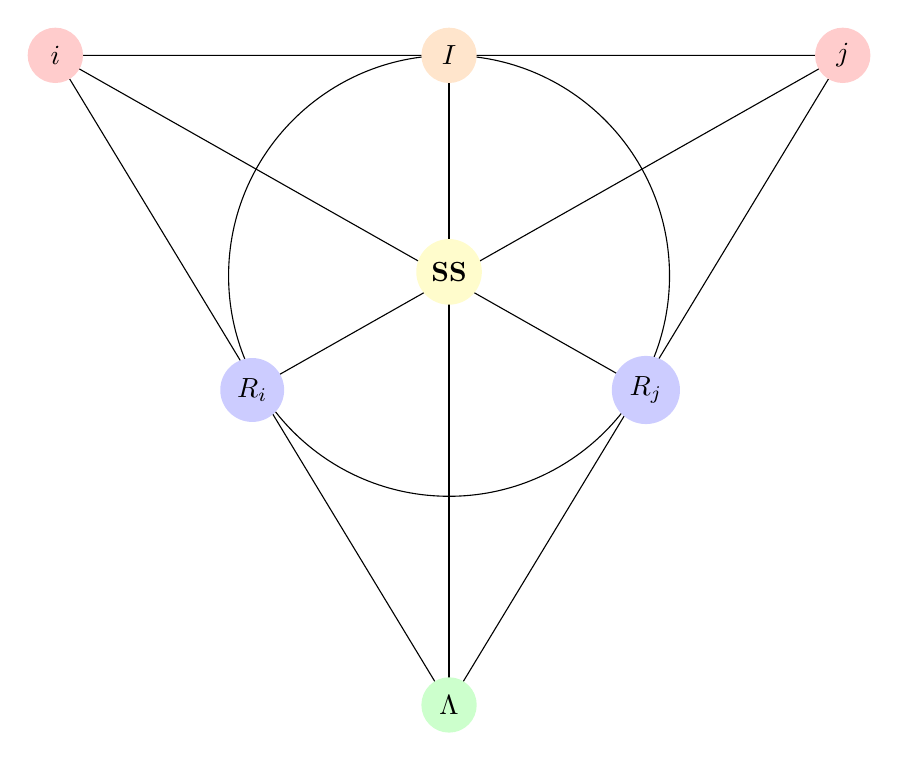
\begin{tikzpicture}[scale=0.5]
\draw (0,17) -- (10,0.5) -- (20,17) -- (0,17);
\draw (10,0.5) -- (10,17);
\draw (0,17) -- (15,8.5);
\draw (20,17) -- (5,8.5);
\draw (10,11.4) circle (5.6cm) ;
\draw (10,0.5) node[minimum size=2em,circle,fill=green!20] {$\Lambda$};
\draw (0,17) node[minimum size=2em,circle,fill=red!20] {$i$};
\draw (20,17) node[minimum size=2em,circle,fill=red!20] {$j$};
\draw (10,17) node[minimum size=2em,circle,fill=orange!20] {$I$};
\draw (5,8.5) node[minimum size=2em,circle,fill=blue!20] {$R_i$};
\draw (15,8.5) node[minimum size=2em,circle,fill=blue!20] {$R_j$};
\draw (10,11.5) node[minimum size=2em,circle,fill=yellow!20] {\textbf{SS}};
\end{tikzpicture}
\end{center}
\caption[Tripolar reconstruction of economic interaction]{Tripolar reconstruction of economic interaction}
\label{fig:governance}
\end{figure}

Consider a population of consumer-producers given by the set $N$, whereby two agents $i,j \in N$ are willing to engage in some mutually beneficial bilateral economic interaction under a governance system, denoted by $\Lambda$. The two agents alone are are unable to engage in a functional wealth generating relationship without the use of accepted institutions that are common knowledge for both agents. These institutions guide actions that resolve issues regarding the final distributions of Core allocations in trade. Without institutions problems with the indeterminancy of contract exist, which obstructs any possibility for exchange to take place. In this way economic agents are fundamentally opposing forces and require a governance system to facilitate exchange. Due to their centripetal and centrifugal forces, these three elements---the two economic agents and the overarching governance system---comprise the three poles of the tripolar model. 

In order to generate wealth through the formation of an economic relationship each agent must use tools provided by the governance system and, as such, form, or conform to, some socio-economic role. Indeed, all interaction between economic agents is executed through the socio-economic roles that each agent adopts. Due to this requirement, the Fano plane also includes the respective socio-economic roles that each economic agent assumes when interacting with each other: these are denoted by nodes $R_{i}$ and $R_{j}$ for agents $i$ and $j$ respectively.

The relationship between the economic agent and the accepted governance system results in the socio-economic role that she adopts. It is an expression of her embeddedness within the social structure encapsulated by the governance system. In order to form a socio-economic role an economic agent must take advantage of embedded elements contained within the governance system. The role that she adopts is a \emph{reflection} of her use of the governance system and thus signifies her embeddedness. The embeddedness hypothesis is therefore graphically represented in the construct of the Fano plane by the relationship $i-R_{i}-\Lambda$, for some economic agent $i \in N$. The embeddedness hypothesis---the bi-directional relationship between the economic agent and the elements of the governance system---is shown in Figure~\ref{fig:embeddednessHypothesis}.

\begin{figure}[h]
\begin{center}
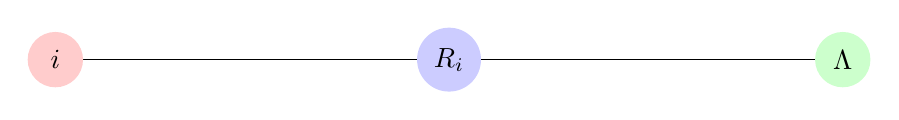
\begin{tikzpicture}[scale=0.5]
\draw (0,0) -- (20,0);
\draw (20,0) node[minimum size=2em,circle,fill=green!20] {$\Lambda$};
\draw (0,0) node[minimum size=2em,circle,fill=red!20] {$i$};
\draw (10,0) node[minimum size=2em,circle,fill=blue!20] {$R_{i}$};
\end{tikzpicture}
\end{center}
\caption[Graphical representation of the embeddedness hypothesis]{Graphical representation of the embeddedness hypothesis}
\label{fig:embeddednessHypothesis}
\end{figure}

When consumer-producers, with the use of their socio-economic roles, engage in an economic interaction their exchange leads to a resource allocation that is represented by a stable state. The tripolar model represents the resulting stable state of economic interaction between agents $i$ and $j$ with the \textbf{SS} node. This stable state is the \emph{realised} resource allocation between the interacting economic agents. The existence of a realised interaction between a pair of agents implies that there must also exist an \emph{idealised} interaction. Note in the diagram that there is another relationship between the two agents intermediated by node $I$. This $i-I-j$ relationship represents the idealised interaction, or \emph{interpersonal relationship}, between the two individual agents. This idealised interaction is observed only when interaction is costless and requires no system of governance, which is often depicted by traditional neoclassical economics, which follows the implicit assumption that agents $i$ and $j$ can interact with each other within a market or exchange economy without any requirement of institutions, socio-economic roles, or media in which to coordinate and guide interaction. The difference between the realised stable state and the idealised resource allocation exists due to the costs of interaction. The costs involved include: 
\begin{itemize}
\item[(a)] An \emph{interaction inefficiency} in using elements of the governance system to form an economic relationship with one another; and 
\item[(b)] \emph{Role-building costs} in the development and utilisation of a socio-economic role.
\end{itemize}
We discuss each of these costs in turn.

\subsubsection{Interaction inefficiency}
\label{subsubsec:interactionInefficiency}

\begin{quote}
Ever since Adam Smith, economists have recognized that gains from trade are the key to the wealth of nations. Specialization and division of labor have made possible the improved productivity that arises from technological change, better resource allocation, and specialized production, the key underlying features of modern economies. What economists have not realized until recently is that the exchange process is not costless. Economists still misunderstand key dilemmas of economies and ignore the costs involved in exchange, assuming (as the standard neoclassicists do) that exchange is costless or unproductive (i.e., the classical notion of unproductive labor)... In fact, the costs of transacting are the key to the performance of economies.

\begin{flushright}
Douglass \citet[p.~1320]{North1989}
\end{flushright}
\end{quote}

The costliness of economic interaction is expressed by the relation $I-\Lambda$, which measures the the degree of interaction inefficiency in actual exchange. This is reflective of the deviation between the idealised economic interaction and the realised stable state. Diagrammatically, the length of the $I-\Lambda$ relationship will depend upon the extent of the transaction costs within society. The $I-\Lambda$ relationship reflects the functionality of the governance system and interaction architectures to generate benefits from the interactions it supports. A governance system that guides more productive economic activities, and possesses fewer transaction costs, promotes a convergence between the idealised and actualised stable states of economic interaction. Indeed, a modification of the governance system or an alteration in the institutions that the agents abide by, the realised interaction between agents $i$ and $j$ can change and can converge towards the idealised interaction. However, there will always be a cost to structuring and following a governance system and, as such, there always exists interaction inefficiencies.

The inefficiency of exchange plays an important role in the discussion of economic interaction with institutions. We therefore make the claim that economic interaction and the formation of functional social and economic relationships are never costless. Regardless of how well-defined a governance system is, there must always exist some interaction inefficiency when using elements of the governance system and subsequently forming functional wealth generating interactions with other economic agents. We denote this interaction inefficiency---the transaction costs of forming and completing economic interactions---by $\Delta(\Lambda)$, such that $\Delta(\Lambda) > 0$, given the existence of some governance system, $\Lambda$.

The two socio-economic roles, $R_{i}$ and $R_{j}$, and the realised interaction, \textbf{SS}, are the only elements in this construct that are observable and measurable. All other elements remain hidden and are, in principle, unobservable. The trade ends in the point \textbf{SS}, its separation from $I$ will determine the relative (in)efficiency of the interaction. Thus $\Delta(\Lambda)$ is given by the distance of the relationship given by $I-\mathbf{SS}$. The idealised exchange is purely aspirational and thus can never be attained: it will always be the case that $\mbox{\textbf{SS}} \neq I$.

\subsubsection{Role-building costs}

Costs also exist with the formation of a socio-economic role. We term the costs related to the adoption of a socio-economic role as role-building costs, denoted by $\delta_{i}(\Lambda)$ for some agent $i \in N$. These costs are graphically represented by the distance of the $i-R_{i}-\Lambda$ relation shown in the tripolar model. Again, role-building costs can be reduced through the presence of more well-defined governance systems, but are always non-trivial.

Specifically, the result of an improved institutional structure will lead to a decrease in the costs of interaction and thus the distance between the realised and the idealised stable state from economic interaction. The interaction inefficiency from $\Lambda$, represented by $\Delta(\Lambda)$, and the role-building costs, represented by $\delta(\Lambda)$, are reduced given a more productive set of institutions. Economic agents can alter elements within the governance system and, in some cases, improve interaction by altering either the formal or informal rules of the game through political influence, or by restructuring the organisation of trade. Finally, an individual can reduce trade costs by altering the actions of a socio-economic role through the development of a new technology, or alternatively by creating a completely new socio-economic role supported by the development of a new technology. New roles, institutions, organisational structures, and technologies can be institutionalised within the governance system and therefore embedded if they are subsequently valued and accepted by society as a whole.

We note that the role-building costs attached to the processes of adaptive and objective specialisation differ substantially, and can also differ depending on the structure of the governance system itself. With regards adaptive specialisation, performing a best response without any institutional guidance is a costly process. An economic agent that adaptively specialises needs to perform three main functions to do so: first, the agent needs to gather information regarding the production plans and potential endowments of all other agents within the economy; second, the resulting utility levels given different production plans of the agent and subsequent trade the exchange mechanism given by the governance system need to be educated; and third, the maximal utility the agent could achieve given the production plan and possible trades needs to be selected. Thus, not only are role-building costs high under adaptive specialisation, but all costs are borne on the individual agent.

\medskip \noindent The structure of institutions play a significant role in the interaction efficiencies and role-building costs that are experienced by the economic agents. It has been well researched that changes in the structure of institutions can modify and redistribute the burden of transaction costs. This can be investigated further with the discussion of entrepreneurship. However, within the relational perspective we also place an importance on the role of trust as a phenomenon that directly supports the formation of social and economic relationships and the formation of socio-economic roles. For example, the process of adaptive specialisation depends on the existence of well-defined institutions; but it also depends on trust that extends from the individual economic agent to the existing institutions and society as a whole to support the new role. Only with the existence of trust and well-defined institutions will economic agents embrace the inherent uncertainty and risk of completely specialising a socially unknown or ill-defined role. As such, trust acts as the \emph{dual} to embeddedness\footnote{Although trust plays an important role in the relational perspective of socio-economic activity it is not crucial to our latter discussion of the entrepreneur. We therefore leave an elaborate discussion of trust as the dual of embeddedness to Appendix~\ref{App:trust}.}.

\subsection{Interaction infrastructures}

The formation of economic interactions and relationships through the utilisation of a commonly accepted governance system forms a structure that individual conumer-producers are positioned within. This resulting matrix of relationships forms an \emph{interaction infrastructure} on which to navigate.
\begin{definition}[Interaction infrastructure] \label{definition:interactionInfrastruture}
An \textbf{interaction infrastructure} refers to a tuple consisting of : 
\begin{itemize}
\item[(1)] A population of consumer-producers; and 
\item[(2)] A set of functional economic interactions and relationships formed between the population of consumer-producers.
\end{itemize}
\end{definition} 
Interaction infrastructures are represented as networks that embrace social and economic interactions and relationships. Analysis typically partitions social and economic interactions, meaning that these networks are traditionally investigated independently as discussed in Section~\ref{sec:socialeconomicnetworks}.

As interaction infrastructures grow both weak and strong ties develop between the nodes\footnote{The evolutionary nature of the the human species suggests that we have a natural ability to form social relations with one another: \emph{Homo Sapiens Sapiens}, or \emph{Homo Dictyous} \citep{ChristakisFowler2009}, are social networkers. The formation of networks of social and economic relationships depends on a set of rules and norms that guide society. Indeed, as economic interactions become more sprawling, and unsupported by social relations, there can emerge problems of opportunism and information asymmetries which naturally derive from the division of labour. This is further exacerbated by the boundedness of human intelligence and cognition.}. This ultimately results into a society that is closely knit together in a dense pattern of many social and economic linkages. Research has found that \emph{densification} and community formation is the natural evolution path for social networks \citep{Leskovec2005a, Leskovec2007a, Leskovec2008}. Within dense social networks institutions and systems of governance can be increasingly developed and enforced \citep{North1989, North1990}; furthermore economic interactions and linkages can be formed and sustained.

Further, the nature of the social division of labour claims that tasks can be performed in a structured sequence. This allows the production of complex consumption goods; such goods are realised through intermediate stages performed by distinct specialised individuals. The consequence of the social division of labour is the emergence of a socially supported economic network---or \emph{interaction infrastructure}---whereby individual agents possess positions in the networked architecture. Their position depends on the interactions they are engaged in, which in turn depends on the socio-economic role that they conform to. This leads to the following hypothesis regarding the economic agent.

\begin{lemma}[Positional attributes of economic agents] \label{con:positionalattributes}
Economic agents have a relational position within an interaction infrastructure. These positional attributes are derived from the economic interactions they form with others.
\end{lemma}

We argue throughout the monograph that the economic interactions, and thus the positional attributes, of an economic agent are largely related to the socio-economic role that they form through their specialisation process. Therefore, an agents position in the economy's interaction infrastructure is largely a result of the output that they produce. New socio-economic roles along with new outputs lead to unique positions in the economy.

% Renee : What is the Marxian thesis re discrepancies of wealth which is being referred to?

Discrepancies in wealth naturally emerge as a consequence of heterogeneous specialisation. To this we also note that specialisation can lead to heterogeneous relational and positional network properties, which relate to the economic opportunities that they can engage in. Within a network context some specialisations are more contested than others, and some are more integral to the functioning of the economic network than others. These differences, when investigating emergent strategies on a network, can provide the basis for the perceived discrepancies of wage and wealth between different specialisations. Understanding how an economy is constructed in terms of specialisations and economic relationships, and understanding the dynamics of this construct, can undoubtedly help us understand both microeconomic and macroeconomic phenomena.

\section{Recap on fundamentals of the relational perspective}
\label{sec:fundamentalsRelationalPerspective}

The relational perspective is based on two fundamental axioms. The first is on the bounded human cognition and the potential Knightian uncertainty that can emerge from social and economic interaction, illustrated in Axiom~\ref{ax:boundedrationality}. This leads to a number of fundamental hypotheses based on the organisational principles of economic interaction. Namely, the formation and use of systems of guidance, which leads to the embeddedness hypothesis (Hypothesis~\ref{ax:embeddednesshypothesis}) and the trust hypothesis (Hypothesis~\ref{trusthyp} in Appendix~\ref{App:trust}) to support these systems of guidance. The social structure that develops can be seen as an extension of human nature as described by the social brain hypothesis (Hypothesis~\ref{hyp:socialbrian}).

The second axiom refers to the harmonisation of production and consumption given by Axiom~\ref{dichotomyhype}. This leads to the notions of increasing returns to specialisation (Hypothesis~\ref{IRShyp}) on the production side and gains from trade (Hypothesis~\ref{Gainsfromtrade}) on the consumption side. The hypothesis regarding the social organisation of production (Hypothesis~\ref{hyp:socialorganisationproduction}) is present throughout. These hypotheses lead to derived outcomes, such as the social division of labour (Lemma~\ref{SDoL}) and positional attributes of economic agents (Lemma~\ref{con:positionalattributes}). These axioms and hypotheses are enough to develop a more structured theory of the relational perspective. This is the aim for subsequent chapters.

\medskip\noindent Starting with insights into the nature and evolution of \emph{Homo Sapiens Sapiens} we have built, very briefly, the building blocks of society. The main features were the boundedly rational consumer-producer itself, the governance system as a collection of informal and formal institutions, the roles in which consumer-producers can express, as well as socially recognised organisational or interaction infrastructures, the nexus of trust that acts in a dual nature to the functional relationships between economic agents and the socially constructed governance system, and the social division of labour within which all economic wealth is generated.

These building blocks are contained within some interaction space denoted as a \emph{socio-economic space}. This is a concept explained in detail in the next chapter.

\begin{subappendices}

\section{Consumer-producers in autarky}
\label{App:autarky}

The notion of a consumer-producers combines the individual characteristics of an economic agent into a single mathematical representation. The individualistic characteristics of an economic agent $i \in N$ are now represented as a consumer-producer $(u_{i}, \mathcal{P}_{i})$ consisting of a conventional utility function $u_{i} \colon \mathcal{C} \rightarrow \mathbb{R}$ and an individual home-based production set $\mathcal{P}_{i} \subset \mathcal{C}$ satisfying Axiom~\ref{ax:productionset}. For notational simplicity we equate $i \in N$ and the consumer-producer representation, $(u_{i}, \mathcal{P}_{i})$, such that $i = (u_{i}, \mathcal{P}_{i})$.

Agents are unable to form functional relationships in economies with deficient governance systems and large interaction inefficiencies. As a consequence the interaction infrastructure is empty and agents can only maximise their utility across their own production set. Society exists as a set of independently operating individual economic agents---\emph{monads}---that do not interact with each other in economically meaningful ways. In this organisational form economic agents are fully self-sufficient and use their productive abilities to achieve a subsistence level of economic wealth to survive. This state is of optimisation is denoted as autarky.

The non-existence of socio-economic interaction may be due to the excessively high interaction inefficiency of engaging with other economic agents. It may be that role-building costs---the costs incurred to an economic agent for forming or conforming to a socio-economic role---are too high thus not facilitating the formation of exchange relationships. Generally, as noted in Section~\ref{subsubsec:interactionInefficiency}, the interaction inefficiency is always above zero; the extent to which the interaction inefficiency is above zero depends on the productivity of the institutional framework.

Agents require a degree of rationality under a state of autarky. This assumed rationality is limited to the ability regarding the maximisation of the objective function of the consumer-producer, where the objective function requires knowledge of the agents own preferences and production set. Indeed, a consumer-producer in autarky thus maximises her utility subject to her own production possibilities. Therefore we assume that a consumer-producer has full knowledge regarding her preferences and her production abilities. This optimisation is given by the \emph{autarky problem}.

\subsubsection{Autarky problem}

The autarky problem is given below.
\begin{definition}[Autarky problem] \label{def:autarkyproblem}
Consider a consumer-producer $(u_{i}, \mathcal{P}_i)$ representation of an economic agent. The consumer-producer $(u_{i}, \mathcal{P}_i)$ is in an autarkic state if she solves the following decision problem
\begin{equation}
\max u_{i}(x) \mbox{ subject to } x \in \mathcal{P}_{i} .
\end{equation}
The decision problem formulated is known as the \textbf{autarky problem}.

If all consumer-producers are autarkic then the predominant organisational form is called a \textbf{monadic economy}.
\end{definition}
In autarky, a consumer-producer is fully restricted as a purely individual decision maker who only accesses the resources she has complete control over: her production set. We provide a simple example to the standard autarky problem with a Stone-Geary utility function.
\begin{example} \label{ex:autarky}
Consider a consumer-producer, $i$, given by $(u_{i}, \mathcal{P}_i)$, such that $i = (u_{i}, \mathcal{P}_i)$, and a consumption space characterised by two goods, $X$ and $Y$. The consumer-producer is endowed with a Stone-Geary utility function given by
\begin{equation*}
u_{i}(x, y) = (x + 1)(y + 1) .
\end{equation*}
Now, consider the production set of the agent, given by
\[ \mathcal{P}_{i} = \left\{ \begin{array}{ll}
         x + y \leqslant 0.5 & \mbox{if $x,y > 0$}\\
		 x \leqslant 1 & \mbox{if $y = 0$}\\
         y \leqslant m & \mbox{if $x = 0$}\end{array} \right. \]
If we let $m = 1$, then the autarky problem is solved by the consumer-producer autarkically producing a mixing strategy, such that $(\hat{x}, \hat{y}) = (0.25, 0.25)$ and $\hat{u}_{i}(\hat{x}, \hat{y}) = 2.25$.

If, however, $m = 2$, then the autarky problem is solved when the consumer-producer autarkically specialises in the production of $Y$, such that $(\tilde{x}, \tilde{y}) = (0, 2)$ and $\tilde{u}_{i}(\tilde{x}, \tilde{y}) = 3$.
\end{example}
Example~\ref{ex:autarky} highlights two features. First, if the learning effects for some economic good are large enough then even in the state of nature economic agents can still specialise in the production of a single economic good. Second, the Stone-Geary utility function facilitates this autarkic specialisation into a given economic good which the Cobb-Douglas production function does not.

The monadic economy of autarkic agents is the most rudimentary form of organisation. This organisational form requires no trust in the systems of governance or operational confidence in the socio-economic roles of others. From this we move to a more developed economy with a more difficult optimisation and potentially complex organisational structure. Specifically, we investigate the notion of adaptive specialisation---as discussed in Definition~\ref{formsofspec}---applied to our notion of consumer-producers. Such a form of specialisation requires a higher form of rationalisation.

\section{Trust}
\label{App:trust}

In \emph{The Company of Strangers} Paul \citet{Seabright2009} claims that the ability to interact with strangers has come from more than just the creation of institution based on the foundations of rationality. In his perspective, the development of institutional mechanisms would have not been feasible without humans evolved ability to develop relationships based on trust. It is our purely natural propensity to place trust in other people through the inducement of natural hormones that is the key for initial consent and cooperation, the subsequent development of institutions, and the creation of social and economic networks. Shorn of our ability to place trust in one another society, and the economy as we know it, would cease to exist.

This fundamental trusting behaviour is well documented as an evolved characteristic of human nature that can transcend rationality. Below we discuss this evolved mammalian characteristic of trust and note its importance in all economic interaction. The subsequent establishment of the \emph{trust hypothesis} as the dual concept to the embeddedness hypothesis provides the basis for a more detailed discussion regarding the theory of economic interaction with the use of governance systems and trust in those systems.

\subsubsection{The role of neuroeconomics}

A number of economists and neurologists have investigated how different areas of the brain respond to a given set of decisions and interactions. A strand of this research has focussed on the neurological basis of trust during social interaction. \citet{Zak2004} and \citet{Kosfeld2005} find that the neuropeptide `oxytocin' plays a key role in social attachment, affiliation and cohesion by causing a substantial increase in trust among humans thereby greatly increasing the benefits from social interactions. Through the use of the \emph{trust game} they found that the production of oxytocin in the mammalian brain specifically affects an individual's willingness to accept social risks arising through interpersonal interactions. It is the release of oxytocin that has a central role in general behavioural regulation, particularly in social interactions due to its interconnection with the amygdala; a central component of the neuro-circulatory of fear and social cognition \citep{Kirsch2005}. Indeed, not only does oxytocin provide the innate neurological basis of trust and subsequent social interaction, but its release also reduces fear that is typically experienced in risk-taking during social and institutional interaction.

There seems to be a general consensus in this recent research concerning oxytocin's relationship to trust and social attachment. Not only does it provide the endogenous basis for perceived trust between agents, but it also provides the basis for trustworthiness. Specifically, higher levels of oxytocin are associated with trustworthy behaviour such as the reciprocation of trust and the successive establishment of reputations \citep{Zak2005}.  Moreover, it has been suggested that oxytocin is essentially a physiologic signature for empathy which mediates generosity. More specifically, \citet{Barraza2009} finds that empathetic acts on an individual stimulates pro-social behaviour, increasing oxytocin substantially above baseline levels leading to reciprocated empathetic acts and increased generosity between agents. Indeed, it was empathy in others and fairness that guided social and economic interactions and exchange, not self-interest. On the contrary, self-interest is simply an outcome of the dehumanising process of capitalism: a Marxian take on the evolution of the capitalist economy.

The results of tests on oxytocin and trust require further elaboration; however it is seemingly undeniable that the source of the pro-social attributes of the human species are linked with neural developments. The co-evolution of the frontal lobe and the hypothalamus in the human species is undeniably an outcome of social evolution above all else \citep{DunbarShultz2007}. Theories tended to emphasise the importance of the brain's role in technical competence: skills, innovations, and information retrieval. However, now they increasingly favour the suggestion that it is the computational demands of living in large, complex societies that have had an influence on the evolution of our large brains. There is a specific importance on pair-bonding that extends beyond male-female relationships and facilitates cooperative social interaction. Such complex social interaction within a society requires trust and the evolution of mechanisms of trustworthiness; this is where the requirement for the natural production of oxytocin becomes so vital to the pro-social aspects of the human species.

Socio-economic activity is based solely on the concept of trust. As discussed above, this is not necessarily a radically new notion within the economics literature. However, under new evidence we perceive trust in a new way and subsequently draw a distinction between the notion of trust and the notion of trustworthiness. We suggest that trust is essentially an innate feature of the human species: humans are neurologically built to build and navigate social networks and express trusting behaviour; not only to our own family, but to strangers who appear non-threatening. Trustworthiness is essentially a derived feature of trust and is based on more reputational features of the socio-economic agent; whether it be trustworthiness based on the visual representation of the individual, the actions in which they use to interact, or other's opinions of them. Trustworthiness, and therefore trust, can be suggested to be built through positive direct and indirect reciprocity between agents \citep{Nowak2005}.

Thus as the human brain has evolved so too have the neuromodulators that facilitate the propensity for the species to place trust in the hands of the others. Through the development and release of oxytocin during positive social interaction humans have an innate ability to trust and to develop trustworthiness through reputational mechanisms that facilitate socio-economic exchange. What is important to note here is that trust should not be simply considered as an individually rationalised act; it is an embedded trait. Moreover, it underpins all socio-economic interaction: without trust and trustworthiness there would be no trade. This conclusion provides the basis for the trust hypothesis as a compliment to the embeddedness hypothesis.

\subsubsection{The trust hypothesis}

The trust hypothesis, which expresses our discussion, is stated in Hypothesis~\ref{trusthyp} below.

\begin{hypothesis}[Trust hypothesis] \label{trusthyp}
Social and economic embeddedness---as expressed by the embeddedness hypothesis---and institutional trust form a duality.
\end{hypothesis}

The main assumption on which this framework of the relational perspective is founded is the idea that trust and socio-economic interactions relate to each other as a duality. This compares starkly with traditional approaches in economics that trust is firmly founded in methodological individualism; it is erroneously viewed as purely individualistic and interpersonal.

The trust hypothesis does not distinguish between different forms of trust and trusting and trustworthy behaviour that emerge. This is left to a discussion in the next chapter. Instead the trust hypothesis suggests that being subject to, and accepting, the same governance system implies the presence of a fundamental form of trust and trusting behaviour. Therefore, the existence of economic interactions and trade relationships between economic agents implies the existence of institutional trust, and conversely, the non-existence of economic relationships implies the non-existence or breakdown of institutional trust within a governance system. The inability to form economic relations as a consequence of this breakdown of trust coincides to what we believe to be the source of recessions and depressions.

\medskip \noindent Embeddedness into systems of governance facilitate economic interaction and the formation of relationships of exchange. It is fully accepted that economic gains from interaction derive specifically from the division of labour and the increasing returns to specialisation that it promotes. Embeddedness into a system of governance is reflected in the use of socio-economic roles, which in itself acts as part of the division of labour. We provide a deeper discussion on these concepts below.

\subsection{Trust as the dual of embeddedness}

Building from the trust hypothesis (Hypothesis~\ref{trusthyp}) we suggest that trust supports all social and economic interaction. In order to create functional socio-economic relationships there needs to be trust to facilitates their inducement: without trust in the elements of the governance system and confidence in the socio-economic roles of others, mutually beneficial interactions can not take place. Trust is the adhesive that keeps out economy together; and its roots are both social and evolved.

The insight into the importance of trust is nothing new. Since the writings of Adam Smith, economists have been discussing the importance of trust in the underlying mechanisms of the economy and society. Adam Smith claimed that individuals should have status and remuneration dependent upon how much trust must be placed upon them. 

\begin{quote}
The wages of labour vary according to the small or great trust which must be reposed in the workmen... We trust our health to the physician, our fortune, and sometimes our life and reputation, to the lawyer and attorney. Such confidence could not safely be reposed in people of a very mean or low condition. Their reward must be such, therefore, as may give them that rank in the society which so important a trust requires. The long time and the great expense which must be laid out in their education, when combined with this circumstance, necessarily enhance still further the price of their labour.

\begin{flushright}
\citet[p.~91]{Smith1776}
\end{flushright}
\end{quote}

According to Smith the value of labour is not based only on the market forces of demand and supply, but rather on the trust that we must place on certain roles and professions, and the amount of human capital and specialisation that the role requires. Doctors and lawyers receive high compensation due to the level of trust other agents must place on the functioning of their roles. Indeed, these professions are basically uncontested, meaning that we cannot substitute the relationship and place our trust in the roles of others to perform the same actions.

John Stuart Mill wrote that, ``there are countries in Europe... where the most serious impediment to conducting business concerns on a large scale, is the rarity of persons who are supposed fit to be trusted with the receipt and expenditure of large sums of money'' \citep[p.~132]{Mill1848}. Applying the notion of trust to the issue of transaction costs, or more specifically the time spent investigating one's broker or trading partner, Institutional Economists suggest that high trust societies produce more output than low trust societies because of the reduced frictions to exchange. Indeed, a sufficient amount of trust may be crucial to successful development, as \citet[p.~54]{North1990} writes, ``the inability of societies to develop effective low-cost enforcement of contracts is the most important source of both historical stagnation and contemporary underdevelopment in the Third World.'' A low-trust poverty trap can exist for highly underdeveloped economies whereby there is not enough trust in which to develop and support sustainable socio-economic institutions. A vicious cycle emerges whereby a collapse of trust undermines the functionality of socio-economic institutions leading to a breakdown of economic interaction, exchange, and specialisation. This fall of economic activity weakens trust further, thus sparking the process again.

In Lombard Street, Walter Bagehot described that way in which the City of London had evolved in his time. He detailed the workings of the financial markets and the trust that underpinned them. It was trust in the actions of its operators that facilitated such vast economic and financial complexity. Without trust the system would become highly fragile.

\begin{quote}
[I]n exact proportion to the power of this system is its delicacy I should hardly say too much if I said its danger... When we understand that Lombard Street is subject to severe alternations of opposite causes, we should cease to be surprised at its seeming cycles. We should cease too to be surprised at the sudden panics. During the period of reaction and adversity, just even at the last instant of prosperity, the whole structure is delicate. The peculiar essence of our banking system is an unprecedented trust between man and man: and when that trust is much weakened by hidden causes, a small accident may greatly hurt it, and a great accident for a moment may almost destroy it. 

\begin{flushright}
\citet[p.~87--88]{Bagehot1873}
\end{flushright}
\end{quote}

It is this trust that facilitates such powerful, yet such delicate complexity; and it is the removal of this trust that leads to such catastrophic deterioration of these complex and potentially highly prosperous and efficient systems. According to Bagehot, with efficiency and interdependency built on the foundation of trust comes extreme fragility.

\citet{ZakKnack2001} provide a general equilibrium model of \textit{interpersonal trust} in an effort to determine macroeconomic prosperity and growth. They perceive interpersonal trust as the trust that an individual, specifically an investor in their case, has on the agents and institutions of market economies. It is a form of rationalised trust which is shaped by how the individual perceives the risk of engaging in economic interaction with the other agents and institutions. The authors characterise the social, economic, and institutional environments in which trust will be high, and show that low trust environments do not provide the basis for sustained economic growth. Specifically, they characterise low trust socio-economic environments by ones that facilitate a higher level of  moral hazard, or where cheating is more likely, such as when the social distance between agents is larger, formal institutions are weaker, and social sanctions against cheating are ineffective. Moreover, the amount invested in society decreases as social heterogeneity and economic inequality increases, and when formal and informal institutions are weaker, which ultimately adversely impacts income and growth. In a following paper the authors suggested that institutions be developed that are specifically aimed at building the interpersonal trust that appears to be so vital for economic development \citep{KnackZak2003}. In doing so they suggest that the Government should concentrate on developing polices that concentrate on increased freedom of association through a vibrant and dynamic civil society, the enhancement of contract, the reduction of inequality, and the development of educational systems. All in all, the conclusion is one that is apparent in many institutional studies of economic development that have come since: strengthen the rule of law and reduce inequality to facilitate increased social cohesion, economic exchange and investment.

Recently economists have discussed trust, and the effective breakdown of trust when systems lie on the edge of chaos, as a cause to the financial crisis \citep{Shiller2008, Tonkiss2009}. We can evaluate that it is likely that this is the case. However, much of the discussion on trust remains superficial. Trust is not given much of a definition. Any perspective on trust is one-dimensional in that it is seen as individualised, rationalised, and purely cognitive. They suggest that trust between an individual and an institution or a firm is purely an individual phenomenon---what we suggest below is that trust is not just a phenomenon of the individual, but is a phenomenon that extends, in some sense irrationally, to society as a whole. It is this irrational extension of trust to society as a whole, the notional trust extending throughout all interdependent divisions of labour, which is actually required for mass complexity to emerge. It is the source of great wealth and, potentially, great fragility.

\subsubsection{Trust and trustworthiness}

Trust is a prerequisite for individual and social engagement, as well as the subsequent development of reputation required for depersonalised or anonymous interaction. Without trust, in the most general sense of the word, there can be no functional wealth generating interactions between agents. 

But what exactly is \emph{trust}? Trust as a concept is largely ill-defined and typically perceived as individual and rationalised. \citet{Coleman1990} suggests that trust is nothing more than a form of social behaviour of individuals in a group. In this view trust is subject to choice, and can therefore be reduced to purely rationalised behaviour. Thus, agent $i$ makes a rational decision to trust agent $j$ prior to engaging in an economic interaction. Here trust is construed as part of the interaction decision itself and thus fully individualistic. This rationalised perception of trust aligns itself directly to the concept of reputation and to the notion of \textit{calculative trust} \citep{Williamson1993}; trust and resulting cooperation which is formed as a outcome of rationalised---albeit bounded---decision-making.

\citet{Hardin2006} claims that much of the literature on trust confuses the term with the concept of \textit{trustworthiness}. Under his perception an agents' trustworthiness is a function of their previous successful interaction with others or oneself. It is the trustworthiness of an individual that is linked to the individual and their social reputation which can be accounted for, and thus rationalised. This trustworthiness between persons---founded on reputation and repeated interaction---is witnessed in game theoretic modelling of repeated non-cooperative games. This theory predicts that players settle on a certain equilibrium in which they coordinate their actions to achieve a shared objective, and a resulting equilibrium state can be understood as the result of a coherence to a mutually understood convention. Within this convention, individual players choices can either support it or undermine it. Previous actions build reputations and trustworthiness of these individual players, and as a consequence their behaviour and the evolution of the game becomes predictable and rationalisable. Based on rationalised trustworthiness, players follow the convention in every round, therefore the game evolves as an outcome of the convention.

This game theoretic modelling suggests that once conventions built on reputations emerge some players may be willing to temporarily sacrifice their own payoff in order to maintain the social convention in the long-run to maximise their utility---and, as a by-product, societies utility---in successive rounds. From a purely self-interested perspective, an individual may invest in a strategy to strengthen the state of the economy, and subsequently their reputation, thus receiving a stream of future rewards for it. The conclusion of this game theoretic literature is given by \citet{Fehr2009}; who suggests that trust is a purely individual trait that can be instinctual.

Fehr is correct. The problem of Coleman's definition of trust as a form of rationalised trustworthiness is that it precludes discussion over the fundamental questions about human cooperation in an economy and society. Assuming rationalised trustworthiness does not allow for discussion of the formation of exchange networks nor does it allow for an explanation of how social conventions and institutions emerge in the first instance. Instead, Fehr suggests that we are somehow genetically programmed to be guided by the socio-economic institutions that we rationally trust the most. The rules of the game tend to act as a straight-jacket to the decisions of individuals and thus dictate the progress of the game; no discussions are put forward as to how or why institutions emerge and change through time. The interrelationship between trust and socio-economic institutions is important for their evolution through time.

Hardin disagrees with Coleman's definition of trust as a derivative of reputation and instead argues that trust cannot be understood as a rationalised behaviour, but rather has to be assessed as fully innate to the human species. Trust is not subject to choice, but is inalienably embedded within us. Such a notion fits well with the results of experimental trust games carried out on test subjects \citep{Kosfeld2005, Zak2008}. Indeed, these experiments consistently show that cooperation flourishes in the trust game; the average investor sends a significant share of her endowment, and most trustees reciprocate \citep{Camerer2003}. Moreover, the perspective of Hardin is fully backed by results from neuroeconomic literature which suggest that trust is simply an embedded feature of human nature.

With respect to the entrepreneurial function, it should be noted that trust plays a foundational role. We stress that in order for the entrepreneurial function to be successful within the economy there must be a high level of trust. Not only must an entrepreneur place faith in the institutional mechanisms (the rule of law, the financial system) to support innovation and also on other individuals and socio-economic roles; but the entrepreneur must operate within a cohesive and trusting socio-economic environment. Specifically, the social transaction costs must be relatively low in order for the entrepreneur to operate.

\subsection{Economic interaction with trust}

We consider a representative model of trust and trusting behaviour. This model is inherently connected to the model of economic interaction through the use of a governance system as discussed in Section~\ref{interactionGovernanceSystem} above, specifically taking full advantage of the trust hypothesis as the dual concept to the embeddedness hypothesis.

\subsubsection{Institutional trust as a duality of economic interaction}
% (Axiom~\ref{ax:embeddednesshypothesis})
The embeddedness hypothesis states that all wealth generating economic relationships are formed within the context of an accepted governance system of media and institutions. Economic agents need to use elements contained in the governance system in order to facilitate their relationships, meaning that all trade relies of the operation of these institutional elements.

From the discussion above we noted that there will always exist a difference between the idealised and the realised social and economic interactions. This is so because individual economic agents need to use elements of the governance system in order to interact with one another. Indeed, the idealised interpersonal interaction between economic agents will never emerge. Building from this we reject the notion that agents form and strengthen relationships built on so-called \emph{interpersonal trust}. That is, economic agents do not place trust in the personal characteristics of each other and rationalise expectations from this interpersonal interaction and subsequent reciprocity.

There are two reasons for why we reject the notion regarding the importance of interpersonal trust. First, individuals are restricted in their perceptions to only the outward features and actions of other individuals, and therefore cannot truly develop senses about each other that allow them to know each other fully. Trust can only be informed and build upon the outward features of another person, the signals that person emits, and the actions that the other person undertakes. This reduces the actual trusting of another person to trusting the outward signals and observed actions of that other person.

Second, economic agents rely on social institutions and organisations to support our social and economic interactions. This includes a reliance on the media and institutions that comprise the governance system. To interact with other economic agents one must use elements of the governance system to do so. In the vast majority of interactions we submit ourselves to and abide by these institutional rules to communicate with other members of the exchange. Agents therefore require institutional trust as opposed to interpersonal trust to engage in their economic interactions. Interpersonal trust between agents is therefore only considered an idealised form of trust between agents.

\medskip\noindent In our reconstruction of economic activity we noted that individuals interacted with each others' socio-economic roles to engage in economic interaction and exchange. Agents do not interact with the personal characteristics of each other, but they interact with derived elements of the governance system: embedded socio-economic roles. Indeed, it is the formation and use of socio-economic roles that facilitates the formation of functional economic interactions. This informs the embeddedness hypothesis.

The socio-economic role of $i$, given by $R_{i}$ shows the embodiment of the embeddedness of individual $i$ in the governance system $\Lambda$. In this regard embeddedness itself refers to the construction of such a reflection $R_{i}$ of an agent $i$ in the governance system $\Lambda$ itself. This aspect of embeddedness, discussed above, is denoted as role-building. A socio-economic role is constructed through the assumption of certain elements of the governance system that are available to the economic agent $i$.

To form a socio-economoic role an economic agent must have a substantial amount of institutional trust in the elements of the governance system. Thus, in order to form functional economic interactions and trade relationships with other economic agents a given agent needs to have institutional trust. This insight forms the duality between economic activity and institutional trust, thus confirming the trust hypothesis.

\subsubsection{Reconstructing embedded economic interaction}

Multiple forms of trust exist in economic interaction. In discussing the multiple forms of trust we frame it as the dual of the \textit{tripolar model} seen in Figure~\ref{fig:governance}, and suggest that different forms of trust underpin different types of functional relationship within the economy.

\begin{figure}[t]
\begin{center}
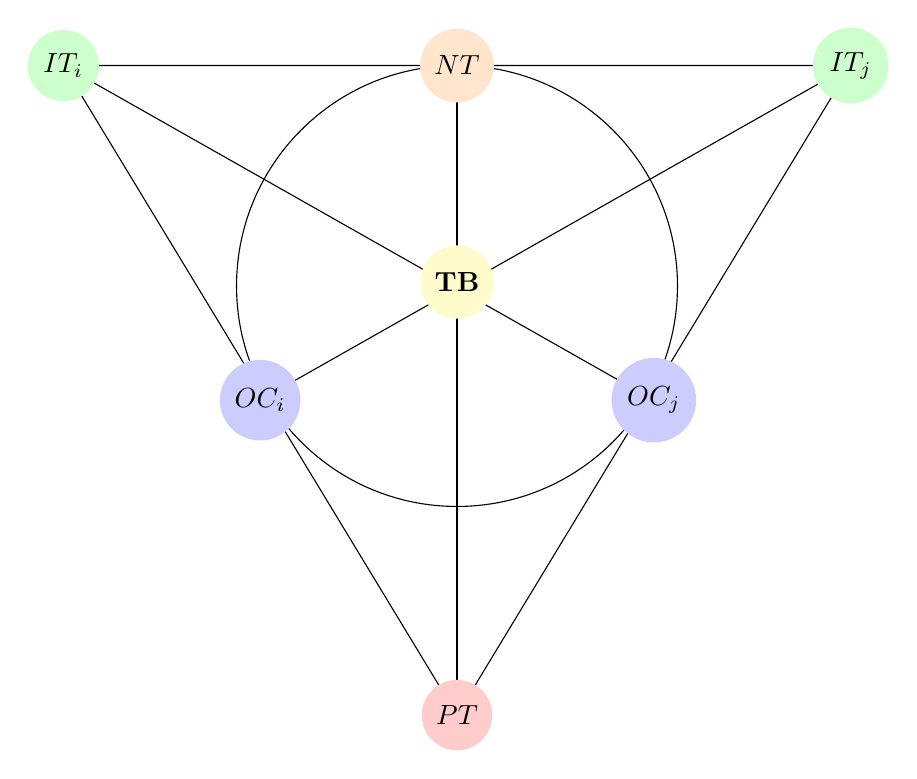
\begin{tikzpicture}[scale=0.5]
\draw (0,17) -- (10,0.5) -- (20,17) -- (0,17);
\draw (10,0.5) -- (10,17);
\draw (0,17) -- (15,8.5);
\draw (20,17) -- (5,8.5);
\draw (10,11.4) circle (5.6cm) ;
\draw (10,0.5) node[minimum size=2em,circle,fill=red!20] {$PT$};
\draw (0,17) node[minimum size=2em,circle,fill=green!20] {$IT_i$};
\draw (20,17) node[minimum size=2em,circle,fill=green!20] {$IT_j$};
\draw (10,17) node[minimum size=2em,circle,fill=orange!20] {$NT$};
\draw (5,8.5) node[minimum size=2em,circle,fill=blue!20] {$OC_i$};
\draw (15,8.5) node[minimum size=2em,circle,fill=blue!20] {$OC_j$};
\draw (10,11.5) node[minimum size=2em,circle,fill=yellow!20] {\textbf{TB}};
\end{tikzpicture}
\end{center}
\caption{Trust as the dual of economic interaction}
\label{dualityoftrust}
\end{figure}

To provide an insight of this dual relation we first discuss the different forms of trust that are inherent within society. Indeed, it is seen that there are three types of trust that hold the functional relationships of society together: interpersonal trust, institutional trust, and notional trust. And two derived forms of trusting behaviour: operational confidence and trust balance. Each of these notions act as the dual to embedded elements and functional interactions explained above. We elaborate on each of these forms of trust and trusting behaviour.

\paragraph{Interpersonal trust ($PT$).}

This is a purely idealised form of trust between the two economic agents, $i$ and $j$. We denote this as an idealised form of trust because agents $i$ and $j$ do not interact with each other at a completely personal level. Indeed, $i$ and $j$ only interact with each other, both socially and economically, with the use of their roles. The two interacting agents simply do not know each other at the most personal and intimate levels needed for interpersonal trust to be realised. No matter how strong the relationship, no two people know each other at an idealised personal level. Indeed, no two people know for certain the incentives, thoughts, and resulting actions of any other person. Increased reciprocity and questioning, i.e. information on the other person, can build a relationship close to the idealised level where interpersonal trust is fully realised, but we must remember that this form of complete trust in one another is purely aspirational and will never be realised in actuality.

In essence, this form of trust acts as the duality of the idealised functional relationship between $i$ and $j$, given by the link $i-I-j$ in Figure~\ref{fig:governance}. Just like this form of trust, the interpersonal functional relationship will never materialise in actuality. Indeed, as we have discussed before, individuals interact with each others' respective socio-economic roles.

\paragraph{Institutional trust ($IT$).}

The relationship of an individual economic agent and the governance system of media, behavioural norms and socio-economic institutions is supported by the trust that each individual has in those elements. This form of trust does not extend to other persons, but rather relates an individual to institutional settings that she observes in her socio-economic environment. This type of trust is denoted as `institutional' trust.

Institutional trust refers to the ability of an individual to use the governance elements to her advantage in her interactions with other individuals. Institutions trust is, in essence, the dual of role-building in that it supports an individuals' attainment of a specific socio-economic role. Indeed, institutional trust is essentially the duality of the functional relationship $i-R_{i}-\Lambda$ and $j-R_{j}-\Lambda$ for agents $i$ and $j$ respectively. Hence why they are seen in the two corners where agents $i$ and $j$ would be. Note, that this form of trust is self-reinforcing: successful role-building leads to an enhancement of the institutional trust that is present within the economy that the agents operate.

We emphasise here that the institutional trust is limited to the relationship of an individual with her institutional environment referred to by the elements in the governance system. In this regard, it has no bearing on the interaction between the two economic agents directly, only indirectly. Indeed, interpersonal trust is essentially individualised and thus only pertains to the agents' interactions with the governance system. However, since the governance system is a social construct, the trust that one places in the governance system only extends to other individuals within society indirectly.

From the discussion of interpersonal trust a form of \textit{derived} trusting behaviour can be attained when assuming that agents are within a social environment---operational confidence.

\paragraph{Operational confidence ($OC$).}

This refers to the confidence that each agent has when using the elements of the governance system to interact with other agents both socially and economically. Operational confidence reflects our institutional trust and our belief that the interaction we pursue in one another can be realised. In an individualised perspective, it simply means that we have the confidence that our roles and actions are understood by society in order to generate successful socio-economic interaction. It is the confidence that our interactions will be successful, thus inferring that our respective roles and actions are valuable.

In a more social perspective, it is the confidence in others: in the roles that other members of society conform to and in the actions that they use to interact. Individuals who do not perform their action in an accepted or recognised way will undermine the operational confidence that others have in them, and thus undermine the functional relationship that the individual has with the rest of society.

Since operational confidence pertains to the interaction that each individual has to each others' socio-economic role, we can suggest that operational confidence is the duality between the relationships $i-SS-R_{j}$ when agent $i$ is interacting with agent $j$'s socio-economic role, and the relationship $j-SS-R_{i}$ when agent $j$ is interacting with agent $i$'s socio-economic role.

\paragraph{Notional trust ($NT$).}

The final type of trusting behaviour to be discussed here is that of notional trust. This form of trust may be considered as an individually \textit{irrational} form of trust in that it is the trust that an individual places on the rest of society as a whole, even when they are not explicitly engaging in any form of interaction with them. It refers to our collective trust in the governance system, in the very media and socio-economic institutions on which a community or society is founded. In some sense this type of trust is the belief that the institutional trust one has is a good proxy for the ideal level of true interpersonal trust. In this respect, notional trust is seen as the duality of the relationship between the governance system and the idealised form of trade: $I-SS-\Lambda$ in Figure~\ref{fig:governance}. Since this is a social---as opposed to a purely individualised---form of trust, we can see that it is diagrammatically placed between the two institutional forms of trust and therefore shared by both individuals within the socio-economic relationship.

Notional trust refers to the claim that all interacting economic agents have common knowledge of all media and socio-economic institutions that lie at the foundation of that environment. In essence, it is notional trust as a fundamental form of social cohesion that is present in any community or society, which facilitates interactions and mutually beneficial exchange. This form of notional trust refers to the very social fabric of the community itself. It refers to the social nature of \textit{Homo Sapiens Sapiens} in the sense that without those media and institutions social behaviour would be impossible. In our lives these social media and skills are hard-wired as much as our desires and abilities are. We grow up in a social environment and the rules of social interaction including language and social habits become part of our inner-most being. As such, notional trust refers to a belief in the social governance system that is part of ourselves.

We can conclude that the trust relationship $IT_{i}-NT-IT_{j}$ is the dual of the governance system itself. In this regard, the governance system is viewed as a ``collective consciousness'' that is accepted and trusted by all members of the society.

\paragraph{Trust balance (TB).}

This is the relationship between the two mutually accepted socio-economic roles and the notional trust. In Figure~\ref{dualityoftrust}, it is the seen as the circular trust relationship connecting to the nodes $OC_{i}-NT-OC_{j}$. It refers to the perception that both economic actors believe that the governance system, and the roles and actions that derive from it, are a good reflection of the idealised interaction that can potentially occur. Disgruntlement over how the governance system affects interaction will lead to a loosening of the trust balance, thus effecting notional trust. Due to this interconnected nature of the nexus of trust, the trust balance is thus a reflection of the other types of trust that maintain economic interaction within society. The poorer condition of the social contract will be reflected in higher transaction costs in which to interact.

Our discussion on trust, and the multiple forms that it can take, should help us capture some notable features of the governance system and economic interaction. First, trust acts in a dual fashion to embeddedness and the functional relationships that subsequently emerge from the mutual use of elements of the governance system. As such without any form of trust in the embedded elements of the governance system, there can be no economic interaction within an economy. Second, it should highlight that all types of trust are essentially interdependent. Indeed, when we see a breakdown in trust we tend to see an unravelling of operational confidence, institutional trust, and thus notional trust throughout society. With this collapse of trust, functional relationships will come to a halt. Given this fact we can see an obvious role for the Government, elites, or entrepreneurs, in rebuilding elements of the governance system to induce trust again and thus facilitating operational trade. With a collapse of trust within the economy we require a reformation of the socio-economic institutions and roles to induce the formation of functional relationships again. Finally, we stipulate that higher levels of trust are required for more complex social and economic interactions. 

\end{subappendices}








% \section{The social division of labour and socio-economic roles}
% \label{sec:SocialDivisionOfLabour}

% The natural argument for the existence of division of labour is the increasing returns generated from the act of specialisation, expressed in Hypothesis~\ref{IRShyp}, and the subsequent gains from trade between these specialised individuals. Gains from trade are traditionally discussed within a macroeconomic context, however this is a notion that is equally applicable within a microeconomic context of specialised exchange. The notion allows for the generation of wealth or surplus from exchange, which is at the heart of classical economic theory. The hypothesis of the natural gains from trade is given by Hypothesis~\ref{Gainsfromtrade} below.
% \begin{hypothesis}[Gains from trade] \label{Gainsfromtrade}
% Simple economic interaction between a pair of specialised economic agents leads to a generation of excess wealth between the two economic agents.
% \end{hypothesis}
% Gains from trade are associated with the consumption abilities of the economic agent and also relate directly to the convexity of the agents utility functions. Gains from trade and the formation of specialised economic interactions require the embeddedness of individual agents and the existence of a social division of labour. The social division of labour suggests that individual economic agents specialise in a communally recognised profession with a corresponding output and use this to exchange with other agents. This is given by Lemma~\ref{SDoL}.
% \begin{lemma}[Social division of labour] \label{SDoL}
% The organisation of social economy is formed as a social division of labour in which individuals execute specialised productive tasks and exchange the resulting outputs from these tasks through socially recognised exchange mechanisms.
% \end{lemma}
% The nature of the social division of labour claims that tasks can be performed in a structured sequence, thus introducing a level of interdependence between the prosperity of economic agents and the generation of wealth throughout society. This allows the production of relatively complex consumption goods; such goods are realised through a sequence of intermediate stages performed by distinct specialised individuals. The ultimate consequence of the social division of labour is the emergence of a socially supported economic network---or \emph{interaction infrastructure}---whereby individual agents possess positions in the networked architecture. Their position depends on the interactions they are engaged in, which in turn depends on the socio-economic role that they conform to. This leads to the following hypothesis regarding the economic agent.
% \begin{lemma}[Positional attributes of economic agents] \label{con:positionalattributes}
% Economic agents have a relational position within an interaction infrastructure. These positional attributes are derived from the economic interactions they form with others.
% \end{lemma}

% We argue below that the economic interactions, and thus the positional attributes, of an economic agent are largely related to the socio-economic role that they form through their specialisation process. Therefore, an agents position in the economy's interaction infrastructure is largely a result of the output that they produce. New socio-economic roles along with new outputs lead to unique positions in the economy.

% \subsubsection{Toward a theory of the division of labour}

% An initial step taken in this monograph to taking Smith's ideas seriously is to embrace the hypothesis that all economic agents are \textit{ex ante} identical with regards their production abilities. As Smith indicates, many differences between specialists that look like \textit{ex ante} differences are in fact \textit{ex post} differences, which emerge due to human capital development as individuals specialise in the production of different outputs. Thus, combining the assumption of \textit{ex ante} identical economic agents with the notion that these identical economic agents can specialise in differentiated outputs with some increasing returns to specialisation; we can add credence to the claim of \citet[p.~43]{BuchananYoon2000} that, ``[e]ven in a world of equals, trade offers mutuality of gain.''

% The assumption that individuals are \textit{ex ante} identical helps to highlight an important merit to of the Smithian framework. In neoclassical theory, if all individuals are \textit{ex ante} identical in all aspects, the economic interaction that emerges will be trivial. But if we use a Smithian perspective we can show that even if individuals are \textit{ex ante} identical in all aspects, \textit{ex post} differences will emerge endogenously from specialisation and the division of labour. This enables interesting stories to be told that cannot be predicted by the neoclassical framework, such as the emergence of middlemen, and hierarchical production organisations. These all result from the evolution of the division of labour, even in the absence of differences between individual agents.

% So, like Smith's original work, and unlike popular perceptions of comparative advantage applied to individual agents, we do not take seriously the assumption that individuals have a natural or exogenous propensity to produce more or high quality output than other individuals. A theory of an exogenous comparative advantage is very logical when applied to regions or nations in models of international trade---some countries do have resource endowments that provide them a comparative advantage over others---but we do not feel that this can necessarily be applied to the individual agent. Smith is taken seriously in suggesting that the increased productivity of the human agent in producing a certain output can come specifically from an endogenous factor: specialisation through learning. This is particularly highlighted in the description of consumer-producers discussed above. 

% Discrepancies in wealth naturally emerge as a consequence of heterogeneous specialisation; which is acknowledged in the Marxian thesis. To this we further note that specialisation can lead to heterogeneous relational and positional network properties, which relate to the economic opportunities that they can engage in. Within a network context some specialisations are more contested than others, and some are more integral to the functioning of the economic network than others. These differences, when investigating emergent strategies on a network, can provide the basis for the perceived discrepancies of wage and wealth between different specialisations. Understanding how an economy is constructed in terms of specialisations and economic relationships, and understanding the dynamics of this construct, can undoubtedly help us understand both microeconomic and macroeconomic phenomena.

% In continuing our discussion of the division of labour we provide an insight into its construct and evolution. In doing so we provide a definition of a \emph{socio-economic role}, which corresponds to a certain well-defined and accepted profession or specialisation within an economy. From this basis, we consider two interlinked concepts, namely \emph{adaptive specialisation} and \emph{objective specialisation}. These notions were initially discussed in a seminal article by \citet{GillesLazarovaRuys2007}. The authors provide a relational model of economic interaction; the non-market environment discussed provides the basis for the emergence of economic trade and specialisation based on the development of socio-economic roles. The concept of specialisation into socio-economic roles is fundamental for the more formal discussion of economic exchange between individual agents provided in this monograph.

% \subsubsection{The social organisation of production}

% From the discussion of the division of labour we can recognise a feature noted by other writers: with the ability to specialise in a variety of productive tasks, agents can be organised in a way to achieve a society that generates collective economic wealth that is subject to increasing returns to scale. This is an outcome given in the hypothesis below.

% \begin{hypothesis}[Social organisation of production] \label{hyp:socialorganisationproduction}
% Production is based on the idea that through an appropriate social organisation individual human productive abilities---being subject to increasing returns to specialisation---can be employed to achieve a social economy that generates collective economic wealth that is subject to increasing returns to scale.
% \end{hypothesis}

% The organisation of the social economy refers to the division of specialised tasks among individuals. It refers to the social organisation of a community to create an economy that is collectively subject to increasing returns in its productive abilities. This is achieved through a social division of labour and forms the foundation of any human society. Within this social organisation individuals perform specialised tasks that are recognisable by all members of the society as socially acceptable and economically viable.

% Specifically, the outputs from the specialised tasks need to be distributed among all members in a socially recognised fashion. This is a conclusion that suggests that a social division of labour requires a supportive social structure or governance system. Economic agents are embedded within a social system. The embeddedness of economic interaction is fundamental to our understanding of the socially structured economy. As a consequence all economic exchange through the productive tasks of the social division of labour depends on this system of institutions.









% \subsubsection{The persistence of governance}

% Some form of the governance system is always needed. Even in the most primitive of civilisations a socially recognised system of rules---even if they are as basic as shared emotions or empathy---is required to facilitate the formation of social relationships. Institutional existence and development are a natural consequence of the evolution of the social brain, oxytocin and the FOXP2 gene which facilitates language and speech \citep{FOXP22002, Tomasello2010}.

% The existence of a social division of labour requires institutional systems to support it. As noted by \citet{Hayek1945} it is the deepening of the division of labour that naturally leads to asymmetric information, knowledge, opportunity throughout the economy; and ultimately the development of mechanisms to structure and guide economic interactions. The division of labour and consequential exchange leads to situations of agency, whereby the information gap between the agents depends on the complexity of the actions carried out by the socio-economic role of each agent. The problem of agency is further exacerbated by the complexity and length of the economic interaction infrastructures that provide commodities to consumers.

% The deepening of the division of labour necessitates the development of institutional structures that permit individuals to take actions that involve complex relationships with other individuals over time. The evolution of increasingly complex interaction structures will not occur if such systems of governance cannot reduce the uncertainties associated with such situations. Institutional reliability is essential; it means that even as the network of interdependence caused by the growth of specialisation widens economic agents can have confidence in outcomes that are necessarily increasingly remote from our personal knowledge. The uncertainty of exchange is removed. This is very much an institutional argument: as the complexity of exchange increases and the interdependent division of labour deepens, there is a necessity for a third party or set of rules in which to initiate institutional mechanisms and reduce the implicit costs of trade. It is the formation of institution, built from trust-building reciprocated interactions \citep{Gintis2000, BowlesGintis2004}, that is required for cooperative behaviour and the generation of wealth. Indeed, we can build a sense of trustworthiness and confidence in the outcomes and operations of others which allows us to engage in wealth-generating interaction.

% We acknowledge that individual agents have an inherent centrifugal force: although they are endowed with both notional production and consumption abilities, it is not necessarily natural to engage in trade with strangers---those outside of an individuals' tightly-knit social network---without some form of mutually accepted centripetal force. Indeed, a centripetal force is required for the notional production and consumption possibilities to become actualised. We advocate that this centripetal force is a socially accepted and embedded governance system to which agents follow in order to engage in socio-economic interaction.

% \medskip\noindent Below we give a clear definition of this socially embedded governance system. After providing definition to the concept and seeing how it relates to the interaction of agents and interaction structures, we structure the governance system and interaction using the governance system within the context of a \textit{tripolar} model. From this, it should become clear that there are costs---whether they be economic or non-economic---to accepting, using, and potentially altering elements of the governance system. Therefore, there are explicit costs to the formation of economic interactions and relationships. This interaction inefficiency will always be the case: exchange can never be idealised, and therefore costless\footnote{We need look no further than the excellent discussions provided by \citet{Coase1937, Coase1960} on the ubiquitous presence of transaction costs.}.